\documentclass[conference]{IEEEtran}
\IEEEoverridecommandlockouts
\usepackage{cite}
\usepackage{amsmath,amssymb,amsfonts}
\usepackage{algorithmic}
\usepackage{graphicx}
\usepackage{textcomp}
\usepackage{xcolor}
\usepackage{booktabs}
\usepackage{xurl}
\usepackage{array}
\newcolumntype{L}[1]{>{\raggedright\arraybackslash}p{#1}}
\def\BibTeX{{\rm B\kern-.05em{\sc i\kern-.025em b}\kern-.08em
    T\kern-.1667em\lower.7ex\hbox{E}\kern-.125emX}}

% Figures and tables are generated by `python -m analysis.paper_figures`
% into paper/figures and paper/tables; this file lives in paper/.
\graphicspath{{figures/}{diagrams/}}

\begin{document}

\title{PQ-Shield: An Empirical Framework for\\
Security--Performance Benchmarking of\\
Post-Quantum Cryptography in\\
Real-Time and Streaming AI Inference APIs}

% TODO(authors): replace x@vit.com with real addresses before submission.
\author{\IEEEauthorblockN{Nivitha K}
\IEEEauthorblockA{\textit{School of Computer Science and Engineering (SCOPE)} \\
\textit{Vellore Institute of Technology}\\
Vellore, India \\
x@vit.com}
\and
\IEEEauthorblockN{Manav Prakash}
\IEEEauthorblockA{\textit{School of Computer Science and Engineering (SCOPE)} \\
\textit{Vellore Institute of Technology}\\
Vellore, India \\
x@vit.com}
\and
\IEEEauthorblockN{Shashwat Kumar}
\IEEEauthorblockA{\textit{School of Computer Science and Engineering (SCOPE)} \\
\textit{Vellore Institute of Technology}\\
Vellore, India \\
x@vit.com}
\and
\IEEEauthorblockN{Yathaartha Srivastava}
\IEEEauthorblockA{\textit{School of Computer Science and Engineering (SCOPE)} \\
\textit{Vellore Institute of Technology}\\
Vellore, India \\
x@vit.com}
}

\maketitle

% =============================================================================
\begin{abstract}
AI inference APIs are protected almost entirely by classical key exchange and signatures, which a
cryptographically relevant quantum computer (CRQC) could break retroactively: traffic recorded today
could be decrypted later (harvest-now-decrypt-later, HNDL). We present PQ-Shield, an application-layer
emulation of protected inference transactions that wraps a real FastAPI service in six configurations:
Control, Classical-RSA (RSA-2048-OAEP with per-transaction key generation, a legacy worst case),
Classical-ECDHE (X25519), Hybrid (ML-KEM-768 with ECDSA), Hybrid-KEX (X25519MLKEM768 with ECDSA), and
Full PQC (ML-KEM-768 with ML-DSA-65). We measure them under concurrency, four payload shapes,
byte-level network emulation, session reuse, and active and passive attacks, with streaming responses
from a real Llama-3.2-3B model, and separate cryptographic from protocol overhead with a matched
no-crypto control. Relative to that control, the cryptographic overhead at 10 connections is
1.3--2.7\,ms per 92\,ms transaction for Full PQC, Hybrid, and Classical-ECDHE, and Hybrid and Full PQC
are statistically equivalent to X25519 within $\pm5\%$ at 10 and 1,000 connections; in our emulation
of a 100\,ms, 5\,Mbit/s path, ML-KEM adds about 5\,ms of handshake time. Per-chunk post-quantum
signing, not key exchange, is the expensive case: we treat per-chunk and hash-chained signing as
endpoints of a hash chain checkpointed every $k$ chunks and measure the trade-off between signature
bytes and \emph{exposure}, the tokens shown before verification (ML-DSA-65: 135,669\,B at $k{=}1$,
3,309\,B at $k{=}\infty$ per 200 tokens). Binding session context and a signed end record into the
stream lets every tested drop, reorder, duplication, replay, and truncation attack be detected. Under
classical key exchange a future CRQC could recover 5.8 bytes of plaintext per streamed token; under the
modeled attack, ML-KEM-based key establishment exposes none. The ML-KEM bindings reproduce all tested
NIST ACVP outputs byte for byte, and ML-DSA verification gives the expected verdict on all tested
vectors.
\end{abstract}

\begin{IEEEkeywords}
post-quantum cryptography, ML-KEM, ML-DSA, hybrid key exchange, harvest-now-decrypt-later,
AI inference APIs, LLM streaming, stream authentication, benchmarking
\end{IEEEkeywords}

% =============================================================================
\section{Introduction}
AI inference endpoints---hosted by commercial providers, on managed cloud platforms, or as custom
FastAPI/Flask services---carry model inputs and outputs that can be sensitive: diagnostic features,
financial records, and increasingly the full text of conversational and agentic sessions. Inference
endpoints are already a recognised attack surface for interception, tampering, and privacy leakage
\cite{tidjon2022threat,song2019privacy}. Their transport protection rests on RSA or elliptic-curve
key exchange and signatures, all of which Shor's algorithm breaks in polynomial time on a
sufficiently large fault-tolerant quantum computer~\cite{shor1997}. Such a machine does not yet
exist, but the harvest-now-decrypt-later (HNDL) threat means an adversary can record encrypted
traffic today and decrypt it once one does; data whose confidentiality must outlive the arrival of a
CRQC is already exposed~\cite{mosca2018ready,blancoromero2026hndl}.

NIST finalized its first post-quantum standards in August 2024: ML-KEM (FIPS 203) for key
encapsulation~\cite{fips203} and ML-DSA (FIPS 204) for signatures~\cite{fips204}. Protocol-level
migration is under way---the X25519MLKEM768 hybrid group is already negotiated by major browsers and
content-delivery networks~\cite{ietf-ecdhe-mlkem}---and post-quantum TLS has been benchmarked
extensively~\cite{paquin2020benchmarking,sikeridis2020authentication,montenegro2026framework,gomezcambronero2026layered}.
What is missing is an empirical account of what migration costs an AI inference workload
specifically: small structured requests, inference times from milliseconds to seconds, and, for
large language models, responses that are \emph{streamed} token by token and therefore cannot be
signed as a whole before the first byte is sent.

This paper makes seven contributions.
First, a concurrency benchmark (10--1,000 connections, five repetitions per cell) of six
configurations on a real classifier workload, including an X25519 baseline representative of modern
TLS key establishment, the deployed X25519MLKEM768 hybrid, and a matched no-crypto protocol control
that separates cryptographic from protocol overhead, with server CPU and memory and
repetition-level statistics (bootstrap confidence intervals, effect sizes, equivalence tests).
Second, a payload-shape study across four AI workload profiles (163\,B--8\,kB).
Third, network-emulation and session-reuse experiments that bound the cost of post-quantum message
size and quantify how session reuse amortizes key establishment.
Fourth, passive (HNDL) and active (tampering and stream-sequence) threat experiments integrated into
the pipeline.
Fifth, an adaptation of amortized stream signing~\cite{gennaro1997streams,wong1999flows,perrig2000tesla}
to token-by-token LLM responses on a real Llama-3.2-3B backend, where a post-quantum signature's size
(3,309\,B for ML-DSA-65 versus $\approx$71\,B for ECDSA P-256) makes per-chunk signing about forty
times costlier in bytes. We show that naive per-chunk signing admits undetected reordering and
truncation, and close both by binding a role label, the session context, and the chunk index into
every signed message and ending each stream with a signed record of its length.
Sixth, we treat per-chunk and hash-chained signing as the two endpoints of one design space---a hash
chain checkpointed every $k$ chunks---define \emph{exposure}, the number of tokens a client displays
before any signature covers them, and measure signature bytes, exposure, and mid-stream attack
detection for $k\in\{1,2,5,10,20,\infty\}$ against an analytic model that the measurements match
exactly.
Seventh, ground-truth validation of the post-quantum bindings against NIST ACVP known-answer tests
and of the streaming harness against the analytic model.

% =============================================================================
\section{Background and Related Work}

\subsection{Post-Quantum Primitives}
ML-KEM-768 (FIPS 203) is a module-lattice key-encapsulation mechanism at NIST security category 3,
with public key, secret key, and ciphertext sizes of 1,184, 2,400, and 1,088 bytes and a 32-byte
shared secret. ML-DSA-65 (FIPS 204) is a module-lattice signature scheme at the same category, with
public key, secret key, and signature sizes of 1,952, 4,032, and 3,309 bytes. Several publications
that post-date FIPS~204 still quote pre-standardization CRYSTALS-Dilithium3 values (a 3,293-byte
signature and 4,000-byte secret key); all values in this paper are confirmed against FIPS~204 as
finalized (Section~\ref{sec:validation}). The X25519MLKEM768 hybrid~\cite{ietf-ecdhe-mlkem}
concatenates an ML-KEM-768 share with a 32-byte X25519 share and derives the session key from both
shared secrets, so it stays secure unless both algorithms are broken.

\begin{table*}[t]
\caption{Synthesis of related work and the gap each leaves open}
\label{tab:related_work}
\centering
\begin{tabular}{|c|p{5.8cm}|p{6.9cm}|}
\hline
\textbf{Study} & \textbf{Focus} & \textbf{Limitation Addressed Here} \\
\hline
Abbasi et al.~\cite{abbasi2025benchmark} & Heterogeneous-hardware PQC benchmark & No AI workload or network stack \\
\hline
Demir et al.~\cite{demir2025industry} & Industry TLS/telecom PQC deployment & No application-layer API metrics \\
\hline
Egbuagha \& Ikwunna~\cite{egbuagha2025practice} & Protocol-level PQC readiness review & No experimental data \\
\hline
Pote \& Bansode~\cite{pote2025evaluation} & Micro-benchmark of core PQC operations & No web protocol context \\
\hline
Shaw~\cite{shaw2026quantumsafe} & Python X25519+ML-KEM hybrid library & No adversarial threat model \\
\hline
Montenegro et al.~\cite{montenegro2026framework} & Post-quantum TLS 1.3 evaluation framework & Restricted to generic TLS traffic \\
\hline
Chhetri et al.~\cite{chhetri2025survey} & Quantum-safe migration survey & Qualitative; no performance data \\
\hline
Faval et al.~\cite{faval2026mobile} & PQC in 5G core networks & Telecom-specific profiles \\
\hline
Kudaloor \& Aijaz~\cite{kudaloor2026sixg} & PQC for 6G wireless nodes & No REST/JSON API pipeline \\
\hline
Song et al.~\cite{song2019privacy} & Privacy risks of robust ML models & Pre-dates practical PQC standards \\
\hline
Tidjon \& Khomh~\cite{tidjon2022threat} & Threat assessment for ML systems & Ignores transport-layer crypto \\
\hline
Ahmed et al.~\cite{ahmed2025libraries} & PQC support in crypto libraries & No end-to-end measurement \\
\hline
Blanco-Romero et al.~\cite{blancoromero2026hndl} & Economic feasibility of HNDL & No application-layer context \\
\hline
G\'omez-Cambronero et al.~\cite{gomezcambronero2026layered} & Layered TLS 1.3 handshake performance & Fixed key exchange; no signature sweep \\
\hline
Schemitt et al.~\cite{schemitt2025blockchain} & PQC signatures on blockchains & Domain-restricted to blockchain \\
\hline
\end{tabular}
\end{table*}

\subsection{Related Work}
Table~\ref{tab:related_work} synthesizes fifteen studies spanning heterogeneous-hardware PQC
benchmarking, industry deployment, layered TLS 1.3 evaluation, migration surveys, 5G/6G integration,
ML threat modeling, and HNDL economics. None combines AI-specific payload profiling,
application-layer load sweeps, and integrated adversarial experiments, and none addresses streaming
response signatures. Three further lines of work bear directly on our design.

\paragraph*{Post-quantum TLS under network conditions}
Paquin \emph{et al.}~\cite{paquin2020benchmarking} benchmarked post-quantum key exchange and
signatures inside TLS 1.3 over emulated links (Linux \texttt{netem}), showing that on lossy or
low-bandwidth paths message size, not computation, dominates handshake latency. Sikeridis
\emph{et al.}~\cite{sikeridis2020authentication} reached a similar conclusion for post-quantum
authentication, and Montenegro \emph{et al.}~\cite{montenegro2026framework} and
G\'omez-Cambronero \emph{et al.}~\cite{gomezcambronero2026layered} extend the analysis to layered TLS
and application-level load. These works measure the TLS handshake with generic payloads. PQ-Shield
instead measures an application-layer protocol around AI inference payloads, including streaming
responses, and adds controlled adversarial experiments. Our network emulation
(Section~\ref{sec:netem}) is deliberately coarser than theirs---it shapes the byte stream rather than
packets---and we use it to bound, not replace, their packet-level results.

\paragraph*{Stream authentication}
Signing a stream that is not available in full when transmission starts is a classical problem.
Gennaro and Rohatgi~\cite{gennaro1997streams} chain per-block hashes so that one signature
authenticates an entire stream; Wong and Lam~\cite{wong1999flows} amortize one signature over a flow
with hash trees; TESLA and EMSS~\cite{perrig2000tesla} trade immediate verification for low
per-packet overhead. Our hash-chain strategy is an instance of this family, not a new construction,
and inherits the same trade-off: integrity is confirmed only when a signature arrives. What is new is
the setting. LLM token streams have a small, latency-critical first chunk and, with post-quantum
signatures, a per-signature cost large enough that the choice of amortization decides whether
streaming is affordable at all; we make that choice explicit and measurable through checkpointing
(Section~\ref{sec:checkpoint}).

\paragraph*{Side channels in encrypted LLM streams}
Weiss \emph{et al.}~\cite{weiss2024keylogging} recovered the content of encrypted AI-assistant
responses from the sizes of streamed packets (the token-length side channel). The attack is
orthogonal to the key exchange and applies to every protected configuration here, but it sharpens one
qualification: per-chunk and hash-chained signing emit one record per chunk and therefore expose
chunk count and timing, which only buffer-and-sign hides.

% =============================================================================
\section{Threat Model}\label{sec:threats}

\subsection{Harvest-Now-Decrypt-Later (HNDL)}
A passive adversary records every cryptographic artifact on a protected connection---the
key-establishment blob, every AES-256-GCM (nonce, ciphertext) pair, and any signatures---and stores
them until a CRQC becomes available. We assume AES-256-GCM itself remains secure (Grover's algorithm
only halves its effective key length), so what differs between configurations is whether the recorded
handshake lets the adversary recover the session key. Under Shor's algorithm this holds for
RSA-OAEP and X25519. For ML-KEM-768 and X25519MLKEM768 it does not under currently known quantum
attacks, assuming a correct implementation. This is a statement about the modeled key-recovery attack
on the recorded handshake, not a proof that the protocol resists every future attack; in particular,
our handshake does not authenticate server keys with certificates (Section~\ref{sec:design}).

\subsection{Active Man-in-the-Middle (MITM)}
An active adversary on the wire intercepts a response and flips one byte, either inside the AEAD
ciphertext or inside the signature, and we observe whether and \emph{where} the client rejects it. A
ciphertext flip should be rejected by the AEAD authentication-tag check before the payload reaches the
application; a signature flip is caught only when the signature is verified. We log the detection
layer and the time of the rejecting check itself, which separates configurations that merely detect
tampering from those that detect it cheaply and early.

\subsection{Streaming-Specific Threats}
Two threats appear only when one connection streams many chunks. The first is a
\emph{sequence-integrity attack}, in which an on-path adversary rearranges validly protected records
without forging any: it may drop a chunk, reorder two chunks, duplicate a chunk, substitute a validly
signed chunk recorded from \emph{another} session (cross-session replay), or truncate the stream by
cutting it off before its last chunks and its terminal record (forged termination). Each chunk's AEAD
tag and, under naive per-chunk signing, its signature remain valid, so detection requires binding
every signed message to its role, its session, and its position, and authenticating the end of the
stream. Our protocol binds a 3-byte role label, a 32-byte session context derived from the handshake
identifier (one stream per handshake, so it also identifies the stream), and the chunk index into
every signed message, and ends every stream with a signed record that commits to the number of chunks
(Section~\ref{sec:binding}). We measure how early each strategy detects each attack.

The second is \emph{HNDL exposure that compounds with session length}. A streamed session reuses one
session key for every chunk, so a passive adversary who records the handshake captures the whole
session at once: the longer the stream, the more ciphertext becomes retroactively readable the moment
the key exchange is broken. We quantify this by relating the number of generated tokens to the
volume a single future key recovery would expose. None of the evaluated configurations rotates keys
within a session; mid-stream rekeying is left to future work.

% =============================================================================
\section{System Design}\label{sec:design}

\begin{figure*}[t]
\centering
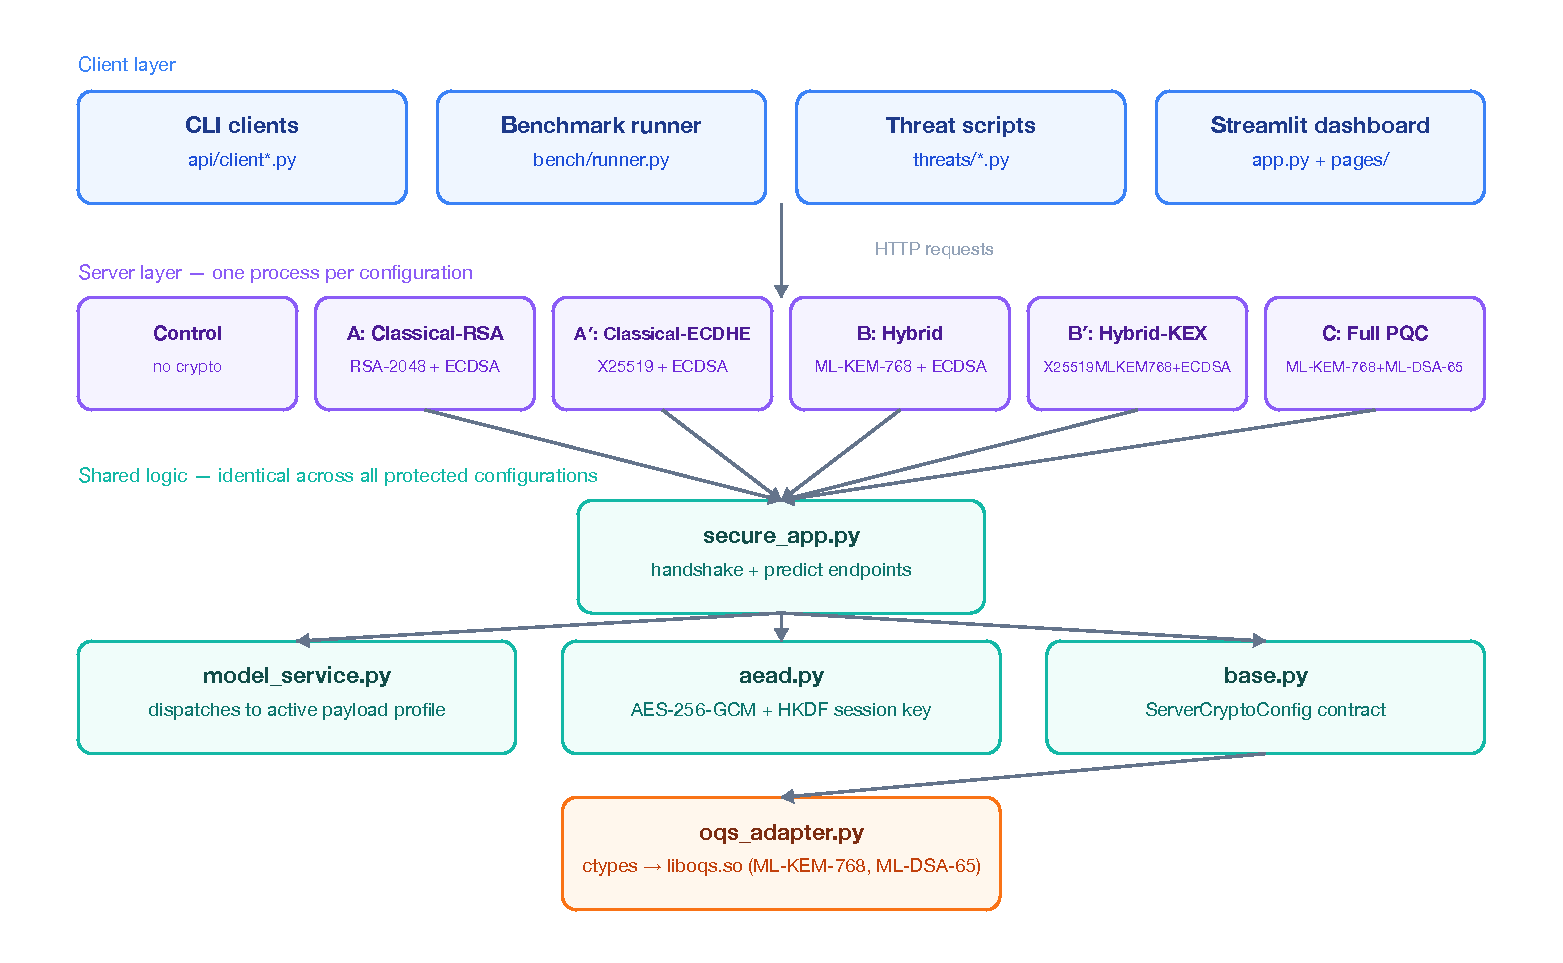
\includegraphics[width=0.85\textwidth]{system_overview.pdf}
\caption{PQ-Shield architecture. Six server processes wrap the same FastAPI inference service: an
unprotected control and five protected configurations that share the handshake/predict endpoints,
the AES-256-GCM + HKDF-SHA256 session layer, and one \texttt{ServerCryptoConfig} contract, so only the
key-establishment and signature primitives differ. ML-KEM-768 and ML-DSA-65 come from a
\texttt{ctypes} binding to liboqs; RSA, X25519, and ECDSA from OpenSSL via the Python
\texttt{cryptography} package.}
\label{fig:architecture}
\end{figure*}

PQ-Shield is an \emph{application-layer emulation of protected inference transactions}, not an
implementation of TLS: it reproduces the cryptographic work of key establishment, payload encryption,
and response signing around an inference call, without certificate authentication or TLS framing.
Six processes wrap the same FastAPI inference server (Fig.~\ref{fig:architecture}): an unprotected
control and five protected configurations (Table~\ref{tab:configs}) sharing a common
\texttt{ServerCryptoConfig}/\texttt{ClientCryptoConfig} contract, so that only the asymmetric
key-establishment and signature primitives differ. All protected configurations use the same
AES-256-GCM layer keyed by HKDF-SHA256 over the raw shared secret. Every protected transaction follows
the same five steps---handshake, session-key establishment, encrypt-and-send, decrypt, verify
(Fig.~\ref{fig:sequence})---with a fresh ephemeral key pair per transaction by default.

\begin{table}[t]
\centering
\caption{Configurations. ECDSA is over P-256; ``PQ'': key exchange resists a CRQC. All protected configurations share AES-256-GCM with an HKDF-SHA256 session key.}
\label{tab:configs}
\setlength{\tabcolsep}{3pt}
\footnotesize
\begin{tabular}{@{}lL{2.6cm}lc@{}}
\toprule
Configuration & Key establishment & Signature & PQ \\
\midrule
Control & none & none & -- \\
A: Classical-RSA & RSA-2048-OAEP (new key per handshake) & ECDSA & no \\
A$'$: Classical-ECDHE & ephemeral X25519 & ECDSA & no \\
B: Hybrid & ML-KEM-768 & ECDSA & yes \\
B$'$: Hybrid-KEX & X25519MLKEM768 & ECDSA & yes \\
C: Full PQC & ML-KEM-768 & ML-DSA-65 & yes \\
\bottomrule
\end{tabular}
\end{table}

Configuration A$'$ is an X25519-based classical baseline representative of the key-establishment
primitive used in modern TLS deployments: TLS 1.3 removed RSA key transport~\cite{rfc8446}, and
ephemeral X25519 is the classical half of the X25519MLKEM768 group now negotiated on the
web~\cite{ietf-ecdhe-mlkem}. A$'$ and B have identical signature code, so
A$'\!\rightarrow$B isolates exactly one change, X25519 to ML-KEM-768. Configuration A uses RSA-2048-OAEP key transport with per-transaction key
generation; no production system generates RSA keys per handshake, so we include A as a legacy
worst-case baseline that exposes the cost of RSA key generation under load, not as \emph{the}
classical baseline. Configuration B pairs a post-quantum key exchange (ML-KEM-768 alone) with a classical
signature. Configuration B$'$ instead combines X25519 and ML-KEM-768 \emph{within} the key exchange,
following~\cite{ietf-ecdhe-mlkem}: the server's share is the ML-KEM encapsulation key followed by an
X25519 public key (1,216\,B), the client's is the ML-KEM ciphertext followed by its X25519 public key
(1,120\,B), and the session key is derived from both shared secrets concatenated. With identical
signature code, A$'\!\rightarrow$B$'$ is the migration step deployed on the web today, and
B$\rightarrow$B$'$ the price of hedging against an ML-KEM break.

Streaming experiments use a real Llama-3.2-3B-Instruct model (Q4\_K\_M, llama.cpp with Metal). The
concurrency, payload-shape, network, session-reuse, HNDL, and MITM experiments use the non-streaming
endpoint with a RandomForest classifier (or the selected payload profile). One locally hosted LLM
produces $\approx$40 tokens per second for a single stream, so a 1,000-connection LLM sweep would
measure the model's queue rather than the cryptography.

\begin{figure}[t]
\centering
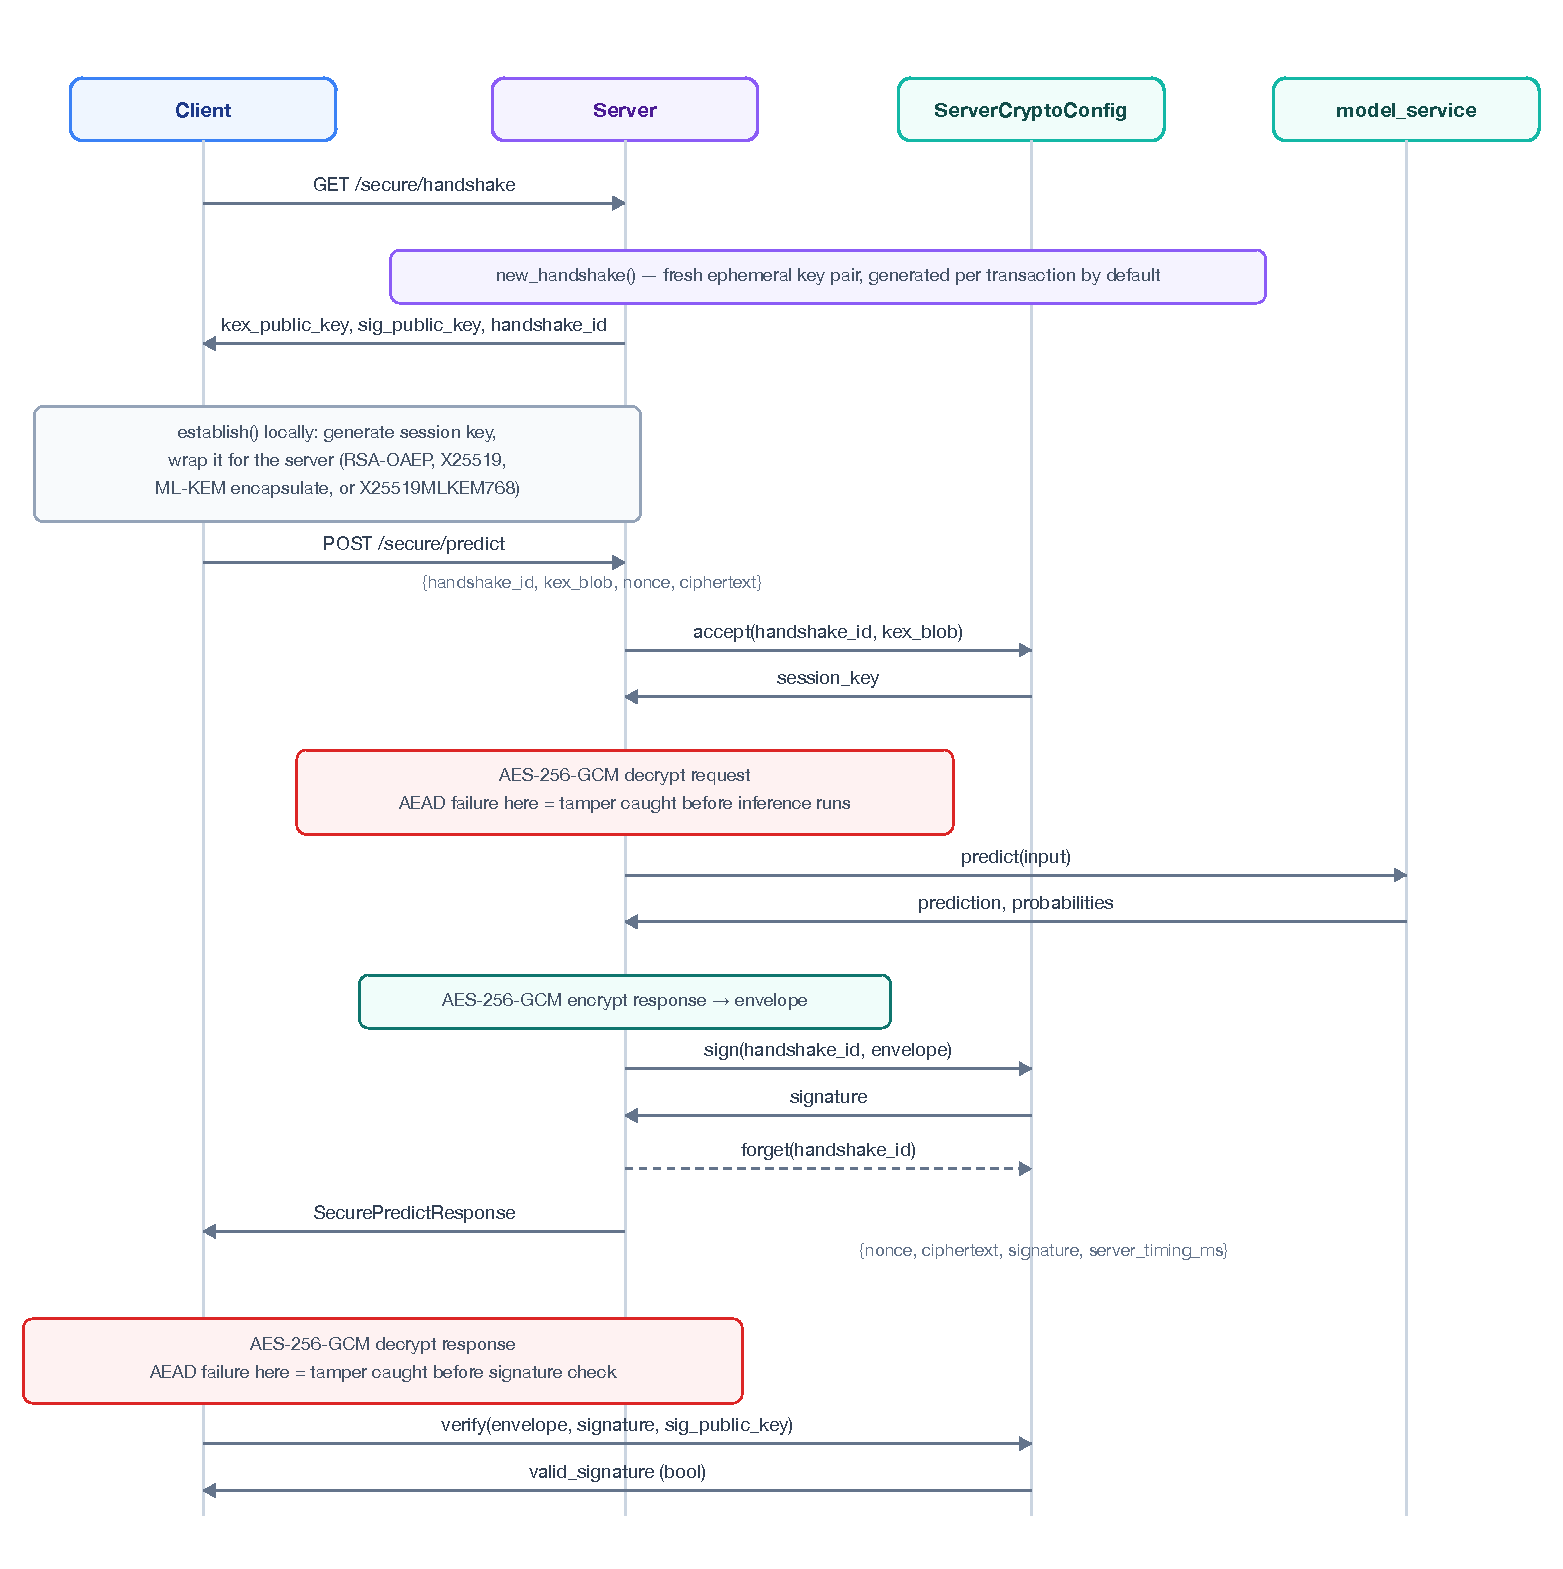
\includegraphics[width=\columnwidth]{transaction_sequence.pdf}
\caption{One protected transaction. The client fetches fresh ephemeral keys, establishes the session
key locally, and sends an encrypted request; the server decapsulates, decrypts (an AEAD failure here
stops tampering before inference), infers, encrypts, and signs. The client decrypts first---an AEAD
failure rejects a tampered response before any signature work---and then verifies the signature.}
\label{fig:sequence}
\end{figure}

% =============================================================================
\section{Methodology}

\subsection{Environment and Process Isolation}
All measurements were taken on one host (Apple M3 MacBook Air, 8 cores, 16\,GB, macOS) on AC power
with low-power mode disabled, on a single day. Each configuration's server runs in its own process,
is health-checked, swept, and stopped before the next configuration starts, so no two configurations
share the CPU. All endpoints, including the control's, run their request handlers in the server's
worker thread pool, so the control is not disadvantaged by blocking inference on the event loop.
Every sweep records a run identifier, the host, and its parameters with each raw row, and the
analysis uses each configuration's most recent run.

\subsection{Cryptographic Binding and Protocol Construction}
ML-KEM-768 and ML-DSA-65 are accessed through a purpose-built \texttt{ctypes} binding against a
locally compiled liboqs~\cite{stebila2016oqs} rather than the higher-level \texttt{liboqs-python}
wrapper. The binding exposes exactly the six C entry points used (key generation, encapsulation, and
decapsulation for ML-KEM-768; key generation, signing, and verification for ML-DSA-65), with byte
lengths asserted against the FIPS~203/204 constants at every call boundary, so a build or linkage
error surfaces immediately rather than propagating malformed key material. liboqs is compiled with
only these two algorithms, which keeps continuous re-verification of the binding
(Section~\ref{sec:validation}) cheap. RSA-OAEP, X25519, ECDSA P-256, and AES-256-GCM come from OpenSSL
through the Python \texttt{cryptography} package.

The handshake orchestration, AES-256-GCM payload encryption (keyed by HKDF-SHA256 over the raw shared
secret in every configuration, including Classical-RSA's OAEP-transported key), and FastAPI plumbing
are identical code paths across configurations, so differences between them can be attributed to the
asymmetric primitives. By default a fresh ephemeral key pair is generated on every transaction---the
conservative worst case; Section~\ref{sec:sessions} measures the amortized case.

\paragraph*{Stream message binding}\label{sec:binding}
For streaming, the same signature primitive is applied to strategy-specific messages, each beginning
with a 3-byte role label and the session context
$\mathit{ctx}=\text{SHA-256}(\texttt{"PQ-Shield-stream-v2"}\parallel\texttt{0x00}\parallel\mathit{hid})$,
where $\mathit{hid}$ is the handshake identifier and $i$, $n$ are 4-byte big-endian integers:
\begin{itemize}
  \item buffer-and-sign: $\mathrm{Sign}(\texttt{BUF}\parallel\mathit{ctx}\parallel\text{nonce}\parallel\text{ct})$;
  \item per-chunk: $\mathrm{Sign}(\texttt{CHK}\parallel\mathit{ctx}\parallel i\parallel\text{nonce}\parallel\text{ct}_i)$
  for every chunk, then a terminal $\mathrm{Sign}(\texttt{END}\parallel\mathit{ctx}\parallel n)$;
  \item hash-chain: $h_0=\text{SHA-256}(\texttt{GEN}\parallel\mathit{ctx})$,
  \begin{equation}
  h_i = \text{SHA-256}(h_{i-1} \parallel i \parallel \text{nonce}_i \parallel \text{ct}_i),
  \end{equation}
  optional checkpoints $\mathrm{Sign}(\texttt{CKP}\parallel\mathit{ctx}\parallel i\parallel h_i)$,
  and a terminal $\mathrm{Sign}(\texttt{FIN}\parallel\mathit{ctx}\parallel n\parallel h_n)$.
\end{itemize}
The role label separates the five message types; $\mathit{ctx}$ makes a record signed for one session
fail verification in any other, even if a server reused one long-term signing key (ours are
per-handshake, which also prevents it); the index binds position; and the terminal records commit to
the stream length. The client requires the terminal record, checks its count against the chunks it
accepted, and recomputes $h_i$ itself rather than trusting transmitted chain hashes.

\subsection{Concurrency Benchmark}
Load is generated by an asynchronous client with a bounded worker pool, so the achieved concurrency
matches the requested level as latency varies. Besides the control (one unprotected request per
transaction) we run a \emph{matched-protocol control}, Control-2RT, which makes the same two HTTP
requests as a protected transaction---a handshake request and the inference request---with no
cryptographic work. Protected minus Control-2RT is then the cryptographic overhead alone, and
Control-2RT minus control the protocol overhead of the extra round trip. Each cell (configuration $\times$ concurrency
$\times$ repetition) sends ten requests per connection (with a floor for low concurrency), and five
repetitions are collected at 10, 100, and 1,000 connections. The first 5\% of requests in each cell
are discarded as warm-up. Latency is end-to-end (\texttt{total\_ms}: handshake round trip plus
protected request), the only quantity directly comparable to the control's single request. A sampler records server CPU and resident memory every 0.25\,s.

\paragraph*{Statistical design} Requests within one repetition share a server process, its warm-up
state, and its queue, so they are not independent; the \emph{repetition} is our unit of analysis. We
report the median, p95, failure rate, and the range of the five per-repetition medians. Differences
between configurations are differences in medians with 95\% confidence intervals from a two-stage
bootstrap (1,000 draws: resample repetitions, then requests within each drawn repetition). Effect
sizes are Cliff's $\delta$. Significance uses the two-sided Mann--Whitney $U$ test on per-repetition
medians (five versus five, so the smallest attainable $p$ is 0.008), Holm-corrected within each
family of comparisons against one reference at one concurrency level. To support claims that two configurations perform the same, we test
equivalence with two one-sided tests: a configuration is declared equivalent to a reference when
the 90\% bootstrap CI of the median difference lies within $\pm5\%$ of the reference median. We call
a difference \emph{practically significant} only if its CI excludes a 5\% band, not merely zero.

\subsection{Payload-Shape Sensitivity}
Four profiles are swept at 10 connections with all six configurations and five repetitions:
\texttt{tabular\_small} (a 100-tree RandomForest trained on the UCI handwritten-digits dataset,
345\,B request / 93\,B response), \texttt{image\_cnn} (a fixed-weight NumPy convolutional network on a
synthetic $32\times32\times3$ image, 4,138\,B / 244\,B), \texttt{embedding} (a synthetic 768-dimension
vector generator, 202\,B / 8,022\,B), and \texttt{llm\_completion} (a synthetic text generator,
163\,B request). The synthetic profiles probe payload shape and size; they are not claims of
representative model behaviour.

\subsection{Streaming Signature Strategies}
The streaming endpoint sends chunks as Server-Sent Events over one HTTP response; each event carries
one strategy-specific record (nonce, ciphertext, and, depending on strategy, a signature and/or chain
hash). The model's blocking token generator is bridged into the server's event loop through a worker
thread so that generation does not stall other requests. Time to first token (TTFT) is measured at
the client from issuing the request to receiving the first event. Each configuration $\times$ strategy
$\times$ length cell (50 and 200 tokens, 5-token chunks) has ten repetitions; after each server start
one discarded generation absorbs the model's cold start, and the order of cells is shuffled with a
fixed seed so that no strategy is always measured first.

\subsection{Checkpointed Hash Chains and Exposure}\label{sec:checkpoint}
The hash-chain strategy can additionally sign the running digest $h_i$ every $k$ chunks. The client
verifies each checkpoint signature against its \emph{own} recomputed $h_i$, so any dropped, reordered,
or altered chunk before a checkpoint makes that checkpoint fail mid-stream. For an $n$-chunk response
this costs $\lfloor n/k\rfloor + 1$ signatures (checkpoints plus the terminal one), and a decrypted
chunk waits at most $k$ chunks for coverage. We record two exposure measures per transaction: the
largest number of chunks displayed but not yet covered by a verified signature (\emph{max unverified
chunks}), and the longest time any chunk waited for coverage (\emph{verification lag}). Per-chunk
signing is the $k{=}1$ endpoint (exposure one chunk) and plain hash-chain the $k{=}\infty$ endpoint
(exposure the whole response). We sweep $k\in\{1,2,5,10,20,\infty\}$ for Hybrid (71\,B signatures) and
Full PQC (3,309\,B) on 200-token Llama responses in 5-token chunks (five repetitions), and at each $k$
repeat the drop and reorder attacks, recording how much of the stream is delivered before detection.

\subsection{Session Resumption}\label{sec:sessions}
To measure the amortized case, a client may set \texttt{keep\_session}: the server then caches the
derived session key under the handshake identifier, later requests carry no key-establishment blob
and reuse it, and the last request of the session ends it. Each of 10 concurrent clients reuses one
key exchange for $N\in\{1,10,100\}$ requests (1,000 requests per cell, five repetitions), and we report
end-to-end overhead against the control.

\subsection{Network Emulation}\label{sec:netem}
All other experiments run over loopback, where moving an extra 1,088-byte ML-KEM ciphertext or
3,309-byte ML-DSA signature costs almost nothing. To expose the cost of message size we place a TCP
proxy between load generator and server that adds a one-way propagation delay of RTT/2 in each
direction and a per-direction bottleneck bandwidth shared by all connections; bytes are released in
order, so HTTP semantics are unchanged. We evaluate four paths---loopback, \emph{metro} (10\,ms RTT,
100\,Mbit/s), \emph{WAN} (50\,ms, 20\,Mbit/s), and \emph{mobile} (100\,ms, 5\,Mbit/s)---each with all six
configurations at 10 connections and five repetitions. The proxy shapes the byte stream above TCP; it
does not model slow start, the initial congestion window, loss, or fragmentation, all of which
penalize large handshakes further~\cite{paquin2020benchmarking}, so the measured cost is a lower
bound.

\subsection{Threat Injection}
For HNDL, the server reports, behind a debug header that does not alter ordinary traffic, the exact
size of each cryptographic artifact it sends (1,000 transactions per configuration). We distinguish
\emph{harvestable} bytes, everything a passive adversary captures (key-establishment blob, AEAD
records, signatures, chain hashes), from \emph{decryptable} bytes, the encrypted application-payload
records whose plaintext becomes recoverable once the session key is recovered. For a stream of $n$
chunks,
\begin{equation}
D = \mathbb{1}_{\mathrm{KEX}}\cdot\sum_{i=1}^{n}\bigl(|\text{nonce}_i| + |\text{ct}_i|\bigr),
\end{equation}
where $\mathbb{1}_{\mathrm{KEX}}$ is 1 if a CRQC can recover the session key from the recorded handshake
(RSA-OAEP, X25519) and 0 otherwise (ML-KEM-768, X25519MLKEM768), $|\text{nonce}_i|=12$\,B and $\text{ct}_i$ includes the 16-byte GCM tag; the recoverable
plaintext is $D-28n$ bytes. Signatures, public keys, and chain hashes are excluded from $D$: they are
not secret. One session key protects the whole stream, and each 5-token chunk is one AEAD record, so
$D$ per token depends on the chunk size (framing) and on the tokenizer (plaintext). For streaming, response length is varied with the
configuration and strategy held fixed, so exposure can be attributed to length alone.

For MITM, a minimal forward proxy flips one bit in either the ciphertext or the signature field of
each response (100 responses per configuration and target). The client decrypts before verifying, and
detection time is the duration of the rejecting step itself---the AEAD tag check or the signature
verification---so the two defence layers are directly comparable. Sequence attacks drop or swap a
mid-stream chunk of a real streamed response and replay the sequence through the client's incremental
verification logic (ten trials per configuration, strategy, and attack).

\subsection{Ground-Truth Validation}
Two independent validations correspond to the two ways this paper's results could be wrong. First,
the primitive bindings are checked against official NIST Automated Cryptographic Validation Protocol
(ACVP) known-answer tests~\cite{acvp} by
re-deriving each vector's output from its input and comparing byte for byte. Second, because no
external dataset exists for streaming signature overhead, the streaming harness is checked against an
analytic model: signature count and bytes follow deterministically from the number of chunks and the
strategy (one signature for buffer-and-sign and plain hash-chain, one per chunk for per-chunk,
$\lfloor n/k\rfloor+1$ for checkpointed hash-chain), and signing time follows from the count and the
independently measured per-signature cost.

\subsection{Reproducibility and Artifact Availability}
Every sweep records its run identifier, host, and parameters with each raw row. The software
environment (OS and package versions, OpenSSL and liboqs revisions, the SHA-256 of the model files,
and the repository commit) is captured automatically at run time and listed in
Table~\ref{tab:environment}. Code, configuration, result summaries, and the scripts that regenerate
every figure and table are released at
\url{https://github.com/Yuvicodes1/PQ-Shield-Benchmarking-Post-Quantum-Security-for-AI-APIs}.

% =============================================================================
\section{Results}\label{sec:results}

\subsection{Cost of Protection Under Concurrency}\label{sec:res-concurrency}
Table~\ref{tab:concurrency} and Fig.~\ref{fig:concurrency} summarize the sweep; differences are
medians with 95\% two-stage bootstrap CIs. At 10 connections the matched-protocol control (Control-2RT)
costs $+1.7$\,ms [$-0.9$, $+4.0$] over the control, so the extra round trip is negligible here, and the
cryptographic overhead (protected minus Control-2RT) is $+1.3$\,ms [$-0.4$, $+3.9$] for Full PQC,
$+2.3$\,ms [$+0.3$, $+5.4$] for Hybrid, $+2.7$\,ms [$+0.8$, $+5.2$] for Classical-ECDHE, $+5.4$\,ms
[$+3.1$, $+8.1$] for Hybrid-KEX, and $+76.8$\,ms [$+67.6$, $+88.6$] for Classical-RSA, against a 92\,ms
transaction. The ML-KEM configurations are statistically equivalent to the X25519 baseline within
$\pm5\%$ (Table~\ref{tab:equivalence}; Hybrid $-0.5\%$ [$-2.1$, $+1.7$], Full PQC $-1.5\%$ [$-3.0$, $+0.2$],
Hybrid-KEX $+2.8\%$ [$+0.8$, $+4.9$]), so replacing X25519 with ML-KEM-768 adds no practically significant
latency in this workload. Classical-RSA's overhead sits almost entirely in the handshake, where the
server generates a fresh RSA-2048 key pair (Fig.~\ref{fig:decomposition}).

At 1,000 connections the four non-RSA protected configurations cost about twice the control
(19.7--20.5\,s against 9.4\,s), but so does Control-2RT (21.3\,s): measured against the matched protocol,
their cryptographic overhead is $-3.7$ to $-7.7\%$, with confidence intervals that include or approach
zero. The doubling is therefore the second HTTP request per transaction, not the cryptography; Hybrid
and Full PQC are again equivalent to Classical-ECDHE within $\pm5\%$. Classical-RSA reaches 30.7\,s
($+44\%$ over Control-2RT) and failures stay at 1.2--1.6\%.

At 100 connections the per-repetition medians of the non-RSA protected configurations are
\emph{bimodal}---each repetition settles near either $\approx$1,000\,ms or $\approx$1,550\,ms (e.g.\
Classical-ECDHE 1,014--1,701\,ms, Full PQC 988--1,604\,ms)---while both controls are stable (Control-2RT
982--1,003\,ms). The resulting overheads have wide intervals (e.g.\ Full PQC $+341$\,ms
[$+38$, $+592$] over Control-2RT), and no ML-KEM configuration can be shown equivalent to, or different
from, Classical-ECDHE at this level. We attribute the regime switching to queueing in a single-host
setup where client and server share the CPU, and do not rank configurations at 100 connections; only
Classical-RSA ($+140\%$ over Control-2RT) is clearly separated.

\begin{figure*}[t]
\centering
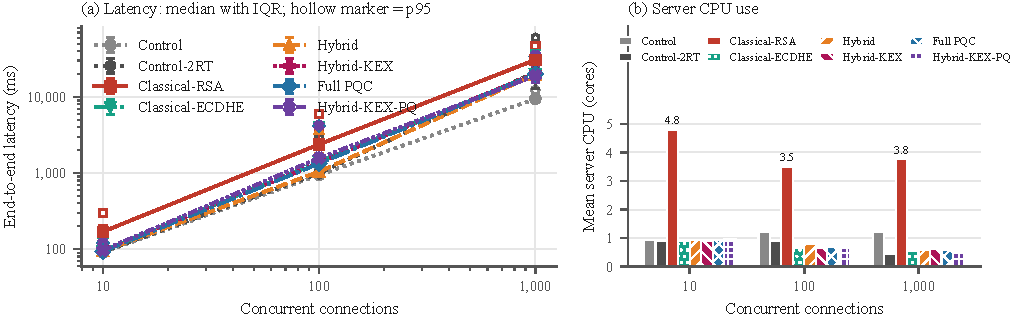
\includegraphics[width=\textwidth]{fig_concurrency_latency.pdf}
\caption{Concurrency sweep. (a) End-to-end latency (median with interquartile range; hollow markers:
p95) on log axes. The four non-RSA protected configurations overlap at every level and, at 1,000
connections, match the matched-protocol Control-2RT; Classical-RSA is consistently slowest. (b) Mean server CPU in cores (100\% = one core): per-handshake RSA-2048 key
generation occupies 3.5--4.8 cores, every other configuration about one core or less.}
\label{fig:concurrency}
\end{figure*}

\begin{table*}[t]
\centering
\caption{End-to-end latency (handshake + protected request) by configuration and concurrency. Statistics over successful requests after 5\% warm-up trimming; ``Rep.\ range'' is the spread of the five per-repetition medians. Overhead and $p$ are versus Control at the same concurrency (two-sided Mann--Whitney $U$).}
\label{tab:concurrency}
\setlength{\tabcolsep}{4pt}
\begin{tabular}{@{}rlrrrrrrrrr@{}}
\toprule
Conc. & Configuration & Reps & OK / attempted & Fail & Median (ms) & Rep.\ range (ms) & p95 (ms) & p99 (ms) & Overhead & $p$ \\
\midrule
10 & Control & 5 & 475 / 475 & 0\% & 90.7 & 89.1--92.3 & 117.0 & 129.9 & ref. & -- \\
 & Classical-RSA & 5 & 475 / 475 & 0\% & 169.2 & 158.2--185.7 & 299.3 & 364.5 & +87\% & $<10^{-135}$ \\
 & Classical-ECDHE & 5 & 475 / 475 & 0\% & 95.2 & 93.7--96.8 & 121.6 & 135.4 & +5\% & $<10^{-6}$ \\
 & Hybrid & 5 & 475 / 475 & 0\% & 94.7 & 93.3--96.2 & 117.5 & 134.1 & +4\% & $<10^{-5}$ \\
 & Hybrid-KEX & 5 & 475 / 475 & 0\% & 97.8 & 96.7--99.8 & 123.4 & 131.8 & +8\% & $<10^{-12}$ \\
 & Full PQC & 5 & 475 / 475 & 0\% & 93.7 & 93.0--94.2 & 120.6 & 140.4 & +3\% & $<10^{-3}$ \\
\addlinespace
100 & Control & 5 & 4,750 / 4,750 & 0\% & 942.9 & 922.8--976.1 & 1,084.1 & 1,175.0 & ref. & -- \\
 & Classical-RSA & 5 & 4,745 / 4,750 & 0\% & 2,381.4 & 2,066.9--2,592.8 & 5,935.1 & 7,242.4 & +153\% & $<10^{-299}$ \\
 & Classical-ECDHE & 5 & 4,746 / 4,750 & 0\% & 1,396.2 & 1,014.0--1,701.4 & 4,081.1 & 5,527.6 & +48\% & $<10^{-299}$ \\
 & Hybrid & 5 & 4,748 / 4,750 & 0\% & 1,043.7 & 983.5--1,590.4 & 3,719.4 & 5,082.7 & +11\% & $<10^{-236}$ \\
 & Hybrid-KEX & 5 & 4,742 / 4,750 & 0\% & 1,361.7 & 1,115.1--1,638.5 & 4,179.9 & 5,510.9 & +44\% & $<10^{-299}$ \\
 & Full PQC & 5 & 4,745 / 4,750 & 0\% & 1,331.9 & 987.8--1,604.3 & 4,139.3 & 5,498.3 & +41\% & $<10^{-299}$ \\
\addlinespace
1,000 & Control & 5 & 47,500 / 47,500 & 0\% & 9,428.0 & 9,402.4--9,586.0 & 12.27\,s & 14.27\,s & ref. & -- \\
 & Classical-RSA & 5 & 46,793 / 47,500 & 1\% & 30.73\,s & 29.94\,s--31.23\,s & 46.42\,s & 61.57\,s & +226\% & $<10^{-299}$ \\
 & Classical-ECDHE & 5 & 46,805 / 47,500 & 1\% & 20.00\,s & 19.57\,s--20.37\,s & 36.62\,s & 46.73\,s & +112\% & $<10^{-299}$ \\
 & Hybrid & 5 & 46,796 / 47,500 & 1\% & 19.66\,s & 19.09\,s--20.10\,s & 34.23\,s & 41.96\,s & +109\% & $<10^{-299}$ \\
 & Hybrid-KEX & 5 & 46,907 / 47,500 & 1\% & 20.52\,s & 19.41\,s--22.53\,s & 35.41\,s & 45.11\,s & +118\% & $<10^{-299}$ \\
 & Full PQC & 5 & 46,740 / 47,500 & 2\% & 19.92\,s & 19.68\,s--20.23\,s & 33.88\,s & 41.73\,s & +111\% & $<10^{-299}$ \\
\bottomrule
\end{tabular}
\end{table*}


\begin{table}[t]
\centering
\caption{Equivalence of ML-KEM-based key establishment to the X25519 baseline (Classical-ECDHE): median end-to-end difference with its 90\% two-stage bootstrap CI, as a percentage of the Classical-ECDHE median. ``Equiv.'': the CI lies within $\pm$5\% (two one-sided tests at $\alpha=0.05$).}
\label{tab:equivalence}
\setlength{\tabcolsep}{3pt}
\footnotesize
\begin{tabular}{@{}rlrl@{}}
\toprule
Conc. & Configuration & $\Delta$ (\%) [90\% CI] & Equiv. \\
\midrule
10 & Hybrid & -0.5 [-2.1, +1.7] & yes \\
 & Hybrid-KEX & +2.8 [+0.8, +4.9] & yes \\
 & Full PQC & -1.5 [-3.0, +0.2] & yes \\
\addlinespace
100 & Hybrid & -25.2 [-43.2, +0.6] & no \\
 & Hybrid-KEX & -2.5 [-27.9, +26.7] & no \\
 & Full PQC & -4.6 [-35.7, +30.3] & no \\
\addlinespace
1,000 & Hybrid & -1.7 [-3.8, +0.6] & yes \\
 & Hybrid-KEX & +2.6 [-1.3, +8.6] & no \\
 & Full PQC & -0.4 [-1.9, +1.0] & yes \\
\bottomrule
\end{tabular}
\end{table}


\begin{figure}[t]
\centering
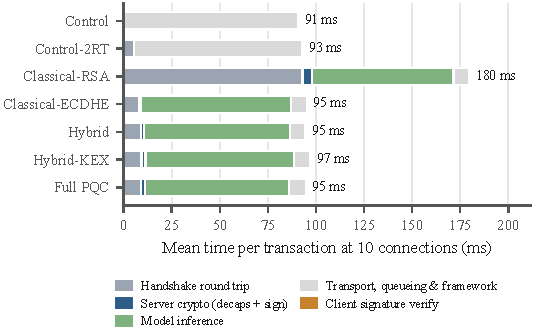
\includegraphics[width=\columnwidth]{fig_latency_decomposition.pdf}
\caption{Mean time per transaction at 10 connections, decomposed. Classical-RSA's extra cost sits in
the handshake (server-side RSA-2048 key generation); for the other configurations the handshake is
$\approx$8\,ms and model inference dominates.}
\label{fig:decomposition}
\end{figure}

\paragraph*{RSA key generation is CPU-bound}
In preliminary runs on a single-core host, Classical-RSA failed every request at 1,000 connections. On
the 8-core host it failed only 1.5\%, while consuming 3.5--4.8 cores of server CPU
(Table~\ref{tab:resources}) against 0.6--0.9 for every other protected configuration. Per-handshake
RSA key generation therefore collapses when cores run out and survives when they do not, at several
times the compute of any alternative. The primitive benchmark explains why: RSA-2048 key generation
runs at 16 operations/s (median 62.7\,ms over 200 samples) against 98,357/s for ML-KEM-768, a
6,167$\times$ gap (Table~\ref{tab:primitives}, Fig.~\ref{fig:primitives}).

\subsection{Server Resources}\label{sec:res-resources}
Apart from Classical-RSA, CPU and memory are flat across configurations: at 10 connections every
non-RSA configuration, including the control, uses 0.92--0.94 cores and 231--241\,MB of resident memory
(Table~\ref{tab:resources}). Post-quantum key and signature sizes did not change memory use appreciably at
this scale.

\begin{table}[t]
\centering
\caption{Server-process resource use, sampled every 0.25\,s during each cell and averaged over repetitions; RSS is mean resident memory (macOS, Apple M3, 8 logical CPUs; 100\% = one core).}
\label{tab:resources}
\setlength{\tabcolsep}{2.5pt}
\footnotesize
\begin{tabular}{@{}rlrrrr@{}}
\toprule
Conc. & Config. & CPU mean & CPU max & RSS & Req/s \\
 & & (\%) & (\%) & (MB) & \\
\midrule
10 & Control & 93 & 126 & 231 & 107.0 \\
 & Control-2RT & 92 & 126 & 231 & 104.4 \\
 & Classical-RSA & 480 & 699 & 238 & 52.4 \\
 & Classical-ECDHE & 92 & 125 & 238 & 101.6 \\
 & Hybrid & 92 & 126 & 239 & 102.1 \\
 & Hybrid-KEX & 92 & 125 & 241 & 99.4 \\
 & Full PQC & 94 & 127 & 241 & 102.1 \\
\addlinespace
100 & Control & 122 & 128 & 241 & 104.8 \\
 & Control-2RT & 92 & 131 & 238 & 78.8 \\
 & Classical-RSA & 351 & 792 & 247 & 35.8 \\
 & Classical-ECDHE & 67 & 134 & 245 & 57.8 \\
 & Hybrid & 80 & 130 & 247 & 68.1 \\
 & Hybrid-KEX & 67 & 132 & 249 & 56.7 \\
 & Full PQC & 68 & 133 & 250 & 58.3 \\
\addlinespace
1,000 & Control & 121 & 129 & 269 & 102.5 \\
 & Control-2RT & 46 & 138 & 214 & 38.4 \\
 & Classical-RSA & 376 & 800 & 283 & 32.9 \\
 & Classical-ECDHE & 56 & 137 & 280 & 46.1 \\
 & Hybrid & 58 & 139 & 286 & 47.7 \\
 & Hybrid-KEX & 64 & 142 & 294 & 45.8 \\
 & Full PQC & 58 & 139 & 290 & 47.7 \\
\bottomrule
\end{tabular}
\end{table}


\subsection{Payload Shape}\label{sec:res-payload}
Across the four profiles the cryptographic overhead is roughly constant in absolute terms
(Fig.~\ref{fig:payload}, Table~\ref{tab:payload}): +4.0--9.4\,ms for every non-RSA configuration and
+71.6--110.2\,ms for Classical-RSA. In relative terms it ranges from +4.5\% for the 89\,ms
RandomForest to up to +240\% for millisecond-scale synthetic profiles. The cost of protection is thus an
additive term independent of payload size; whether it matters depends on the inference time it is
added to. Configurations using X25519 (Classical-ECDHE, Hybrid-KEX) are consistently 1.6--3.5\,ms
slower than those using ML-KEM alone, matching the primitive costs: server-side handshake work is
217.9\,\textmu s for X25519 key generation plus exchange against 23.3\,\textmu s for ML-KEM key
generation plus decapsulation in our implementation.

\begin{figure*}[t]
\centering
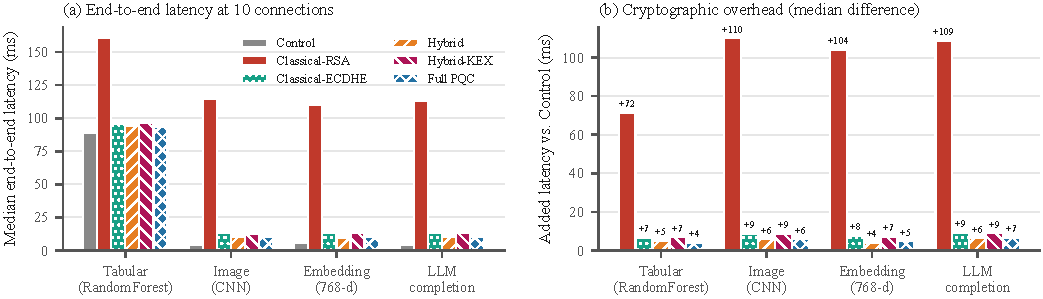
\includegraphics[width=\textwidth]{fig_payload_profiles.pdf}
\caption{Payload-shape sensitivity at 10 connections. (a) Median end-to-end latency per profile.
(b) Added latency versus the control: roughly constant in milliseconds across profiles, so the
cryptographic cost is additive and independent of payload size.}
\label{fig:payload}
\end{figure*}

\begin{table*}[t]
\centering
\caption{Payload-shape sensitivity at 10 connections (5 repetitions per cell). Request/response sizes are plaintext medians; each cell gives median end-to-end latency (ms) and the added latency versus Control, with Mann--Whitney $U$ significance (* $p<0.05$).}
\label{tab:payload}
\setlength{\tabcolsep}{4pt}
\begin{tabular}{@{}lrrrrrrrr@{}}
\toprule
Profile & Req. (B) & Resp. (B) & Control & Classical-RSA & Classical-ECDHE & Hybrid & Hybrid-KEX & Full PQC \\
\midrule
tabular\_small & 348 & 90 & 89.2 & 160.7 (+71.6*) & 95.9 (+6.7*) & 94.3 (+5.1*) & 96.1 (+7.0*) & 93.1 (+4.0*) \\
image\_cnn & 4,138 & 245 & 4.2 & 114.4 (+110.2*) & 13.1 (+8.9*) & 10.2 (+6.0*) & 12.9 (+8.7*) & 10.2 (+6.0*) \\
embedding & 202 & 8,017 & 5.7 & 110.0 (+104.2*) & 13.5 (+7.7*) & 9.9 (+4.2*) & 13.0 (+7.3*) & 10.5 (+4.8*) \\
llm\_completion & 157 & 4,048 & 3.9 & 112.8 (+108.9*) & 13.3 (+9.4*) & 10.3 (+6.4*) & 13.0 (+9.1*) & 10.5 (+6.6*) \\
\bottomrule
\end{tabular}
\end{table*}


\subsection{Network Conditions}\label{sec:res-network}
On emulated paths (Fig.~\ref{fig:network}) the handshake leg isolates the cost of key-exchange size.
Relative to Classical-ECDHE, the ML-KEM configurations add $+4.6\pm0.5$\,ms (Hybrid),
$+4.7\pm0.3$\,ms (Full PQC), and $+5.7\pm1.3$\,ms (Hybrid-KEX) on the mobile path, and at most
1.0\,ms on the metro and WAN paths. End-to-end, these differences are smaller than the
between-repetition variability of server queueing (standard deviation 15--26\,ms on WAN and mobile),
so they are not resolvable at the application level. Classical-RSA's handshake is 61--81\,ms slower
than Classical-ECDHE's on every path because of key generation, not bytes. Because the proxy does not
model TCP slow start or loss, these are lower bounds.

\begin{figure*}[t]
\centering
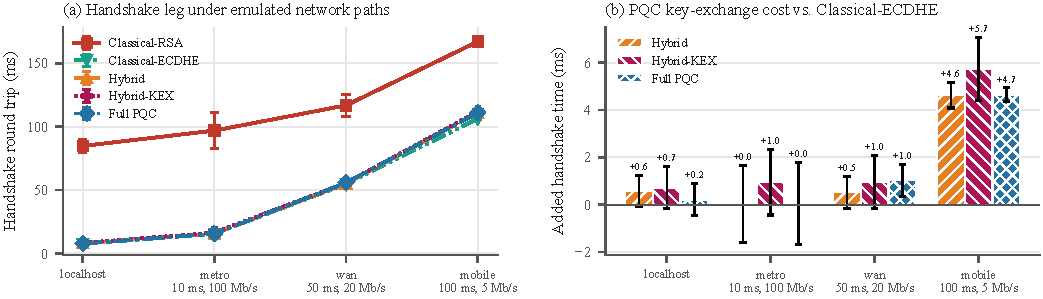
\includegraphics[width=\textwidth]{fig_network_conditions.pdf}
\caption{Emulated network paths (10 connections; mean of five per-repetition medians, error bars one
standard deviation). (a) Handshake round trip. (b) Added handshake time of the ML-KEM configurations
relative to Classical-ECDHE: about 5\,ms on the 5\,Mbit/s mobile path, at most 1\,ms elsewhere.}
\label{fig:network}
\end{figure*}

\subsection{Session Reuse}\label{sec:res-amortization}
Fig.~\ref{fig:amortization} reports overhead versus the control as one key exchange serves $N$
requests. Classical-RSA's +101.2\% at $N{=}1$ disappears at $N{=}10$ ($-1.1\pm1.0$\%). For the other
configurations the overhead falls from +4.0--7.0\% at $N{=}1$ to between $-0.2$ and $+2.1$\% at
$N{=}100$; one intermediate point (Full PQC at $N{=}10$, $+9.0\pm8.4$\%) reflects a single outlying
repetition. For deployments that reuse sessions, post-quantum key establishment cost at most about 2\%
end-to-end in this workload.

\begin{figure*}[t]
\centering
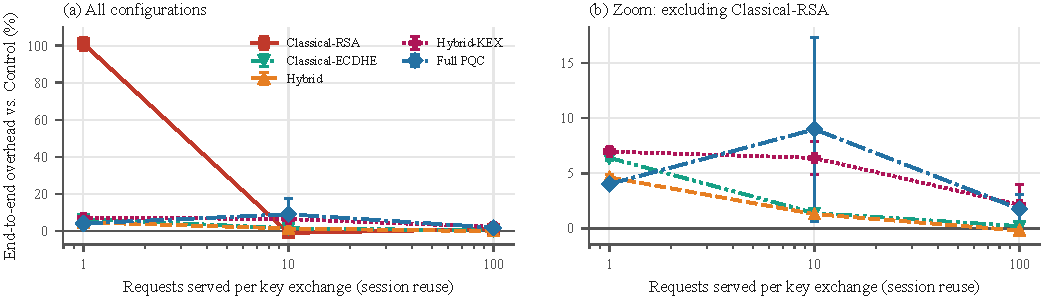
\includegraphics[width=\textwidth]{fig_handshake_amortization.pdf}
\caption{Session reuse at 10 connections (mean $\pm$ one standard deviation over five repetitions).
(a) All configurations: Classical-RSA's overhead vanishes once a key exchange serves ten requests.
(b) Zoom without Classical-RSA: post-quantum overhead falls to 0--2\% at 100 requests per key exchange.}
\label{fig:amortization}
\end{figure*}

\subsection{Streaming Signature Strategies}\label{sec:res-streaming}
With the real Llama-3.2-3B backend (Fig.~\ref{fig:streaming}, Table~\ref{tab:streaming}),
buffer-and-sign delays the first token to the end of generation (5.0--6.1\,s for a 200-token response).
Per-chunk and hash-chain signing both deliver the first token in 126--153\,ms, 38--41$\times$ sooner, in
every configuration. The strategies differ in signature bytes: for Full PQC a 200-token response carries
135,669\,B of ML-DSA-65 signatures under per-chunk signing (40 chunk signatures plus the signed end
record) versus 3,309\,B under hash-chain, a 41$\times$ difference; with ECDSA the corresponding figures
are $\approx$2,910\,B and 71\,B. Within each configuration the strategy order was shuffled, so these
comparisons are unbiased; across configurations, however, generation slowed from $\approx$40 to
$\approx$33 tokens/s over the 18-minute run (thermal throttling of the fanless host), so we do not
compare streaming times between configurations.

\begin{figure*}[t]
\centering
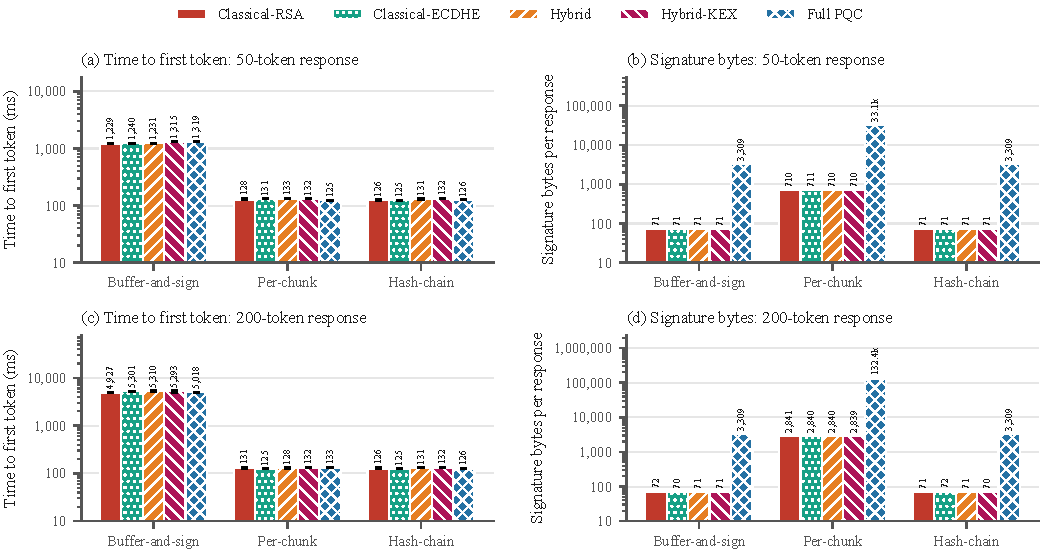
\includegraphics[width=\textwidth]{fig_streaming_strategies.pdf}
\caption{Streaming signature strategies on Llama-3.2-3B (5-token chunks; median of ten repetitions,
error bars interquartile range). (a, c) Time to first token: per-chunk and hash-chain deliver the
first token 38--41$\times$ sooner than buffer-and-sign. (b, d) Signature bytes per response:
per-chunk ML-DSA-65 signing costs 41$\times$ the bytes of hash-chain.}
\label{fig:streaming}
\end{figure*}

\begin{table*}[t]
\centering
\caption{Streaming signature strategies on a real Llama-3.2-3B-Instruct backend (10 repetitions per cell; median, with interquartile range for TTFT). Signing and verification times are summed over the whole stream and given as wall-clock / thread-CPU time; Section~\ref{sec:timing} explains why per-signature cost in a stream exceeds the back-to-back microbenchmark. Generation slowed over the sweep (thermal), so compare times within a configuration, not across.}
\label{tab:streaming}
\setlength{\tabcolsep}{2.4pt}
\footnotesize
\begin{tabular}{@{}rllrrrrrr@{}}
\toprule
Tokens & Config. & Strategy & TTFT (ms) & Total (ms) & Sigs & Sig. bytes & Sign wall/CPU (ms) & Verify wall/CPU (ms) \\
\midrule
50 & Classical-RSA & Buffer-and-sign & 1,239.0 [1,238--1,241] & 1,239 & 1 & 72 & 0.07 / 0.07 & 0.08 / 0.08 \\
 &  & Per-chunk & 126.7 [126--129] & 1,236 & 11 & 780 & 0.43 / 0.44 & 0.74 / 0.74 \\
 &  & Hash-chain & 127.7 [126--130] & 1,239 & 1 & 71 & 0.08 / 0.08 & 0.07 / 0.08 \\
\addlinespace[1pt]
 & Classical-ECDHE & Buffer-and-sign & 1,268.1 [1,256--1,289] & 1,268 & 1 & 71 & 0.07 / 0.07 & 0.08 / 0.08 \\
 &  & Per-chunk & 127.4 [126--129] & 1,262 & 11 & 782 & 0.45 / 0.46 & 0.74 / 0.74 \\
 &  & Hash-chain & 132.8 [130--135] & 1,332 & 1 & 71 & 0.09 / 0.09 & 0.08 / 0.09 \\
\addlinespace[1pt]
 & Hybrid & Buffer-and-sign & 1,313.6 [1,312--1,316] & 1,315 & 1 & 71 & 0.33 / 0.34 & 0.35 / 0.35 \\
 &  & Per-chunk & 136.5 [136--138] & 1,366 & 11 & 781 & 2.55 / 2.59 & 4.57 / 4.56 \\
 &  & Hash-chain & 134.6 [131--136] & 1,350 & 1 & 71 & 0.34 / 0.34 & 0.34 / 0.34 \\
\addlinespace[1pt]
 & Hybrid-KEX & Buffer-and-sign & 1,284.6 [1,280--1,290] & 1,285 & 1 & 71 & 0.07 / 0.07 & 0.08 / 0.08 \\
 &  & Per-chunk & 126.8 [125--128] & 1,241 & 11 & 782 & 0.42 / 0.43 & 0.73 / 0.73 \\
 &  & Hash-chain & 135.6 [135--136] & 1,361 & 1 & 70 & 0.36 / 0.36 & 0.34 / 0.34 \\
\addlinespace[1pt]
 & Full PQC & Buffer-and-sign & 1,298.6 [1,242--1,314] & 1,300 & 1 & 3,309 & 0.46 / 0.47 & 0.22 / 0.22 \\
 &  & Per-chunk & 134.5 [133--135] & 1,366 & 11 & 36,399 & 1.15 / 1.16 & 0.55 / 0.55 \\
 &  & Hash-chain & 133.7 [133--134] & 1,353 & 1 & 3,309 & 0.09 / 0.09 & 0.05 / 0.05 \\
\addlinespace[1pt]
 & Hybrid-KEX-PQ & Buffer-and-sign & 1,322.0 [1,312--1,358] & 1,323 & 1 & 3,309 & 0.43 / 0.44 & 0.26 / 0.27 \\
 &  & Per-chunk & 137.7 [137--140] & 1,387 & 11 & 36,399 & 6.14 / 6.17 & 3.02 / 3.03 \\
 &  & Hash-chain & 137.5 [137--142] & 1,387 & 1 & 3,309 & 0.63 / 0.64 & 0.20 / 0.20 \\
\addlinespace[1pt]
\midrule
200 & Classical-RSA & Buffer-and-sign & 5,053.1 [4,962--5,304] & 5,054 & 1 & 71 & 0.08 / 0.08 & 0.10 / 0.10 \\
 &  & Per-chunk & 128.2 [128--129] & 4,997 & 41 & 2,912 & 1.60 / 1.62 & 2.72 / 2.73 \\
 &  & Hash-chain & 127.0 [127--130] & 4,964 & 1 & 71 & 0.08 / 0.08 & 0.07 / 0.08 \\
\addlinespace[1pt]
 & Classical-ECDHE & Buffer-and-sign & 4,992.2 [4,972--5,024] & 4,993 & 1 & 72 & 0.07 / 0.07 & 0.09 / 0.09 \\
 &  & Per-chunk & 129.8 [127--134] & 5,396 & 41 & 2,912 & 6.78 / 6.80 & 10.00 / 9.93 \\
 &  & Hash-chain & 126.5 [126--127] & 5,025 & 1 & 71 & 0.08 / 0.08 & 0.08 / 0.08 \\
\addlinespace[1pt]
 & Hybrid & Buffer-and-sign & 5,479.0 [5,457--5,495] & 5,480 & 1 & 71 & 0.29 / 0.29 & 0.28 / 0.29 \\
 &  & Per-chunk & 129.6 [129--134] & 5,327 & 41 & 2,908 & 5.29 / 5.34 & 7.83 / 7.85 \\
 &  & Hash-chain & 132.1 [131--133] & 5,393 & 1 & 71 & 0.30 / 0.30 & 0.30 / 0.30 \\
\addlinespace[1pt]
 & Hybrid-KEX & Buffer-and-sign & 5,472.8 [5,416--5,491] & 5,474 & 1 & 71 & 0.34 / 0.35 & 0.28 / 0.29 \\
 &  & Per-chunk & 133.6 [131--135] & 5,523 & 41 & 2,912 & 9.77 / 9.92 & 15.03 / 14.90 \\
 &  & Hash-chain & 127.2 [127--128] & 5,062 & 1 & 71 & 0.08 / 0.08 & 0.08 / 0.08 \\
\addlinespace[1pt]
 & Full PQC & Buffer-and-sign & 5,508.2 [5,488--5,520] & 5,509 & 1 & 3,309 & 0.44 / 0.44 & 0.29 / 0.29 \\
 &  & Per-chunk & 132.2 [130--135] & 5,462 & 41 & 135,669 & 10.91 / 10.99 & 5.89 / 5.83 \\
 &  & Hash-chain & 129.7 [127--132] & 5,246 & 1 & 3,309 & 0.11 / 0.11 & 0.05 / 0.05 \\
\addlinespace[1pt]
 & Hybrid-KEX-PQ & Buffer-and-sign & 5,524.3 [5,356--5,577] & 5,525 & 1 & 3,309 & 0.32 / 0.33 & 0.23 / 0.23 \\
 &  & Per-chunk & 136.5 [133--139] & 5,625 & 41 & 135,669 & 16.25 / 16.33 & 7.59 / 7.64 \\
 &  & Hash-chain & 138.9 [137--143] & 5,614 & 1 & 3,309 & 0.47 / 0.47 & 0.27 / 0.27 \\
\addlinespace[1pt]
\bottomrule
\end{tabular}
\end{table*}


\subsection{Bounded Exposure with Checkpointed Hash Chains}\label{sec:res-checkpoint}
Fig.~\ref{fig:checkpoint} and Table~\ref{tab:checkpoint} sweep the checkpoint interval $k$. Signature
bytes follow the analytic model $(\lfloor n/k\rfloor+1)\cdot|\sigma|$ exactly: for Full PQC 135,669\,B
(41 signatures) at $k{=}1$, 29,781\,B at $k{=}5$, 9,927\,B at $k{=}20$, and 3,309\,B at $k{=}\infty$; for
Hybrid $\approx$2,913\,B to 71\,B. Exposure grows as bytes fall: the client displays at most 5, 25, 100,
and 200 tokens before a signature covers them, with maximum verification lags of 0\,ms, about 0.6\,s,
2.6\,s, and 5.6\,s (Full PQC). The attack experiments show the security effect directly. Without
checkpoints, hash-chain detects every mid-stream drop and reorder but only at the end of the stream.
With checkpoints every drop and reorder is caught mid-stream (100\%), after 50--51\% of the stream at
$k\le2$ (the attack position itself), 59--60\% at $k{=}5$, 72\% at $k{=}10$, and 97--98\% at $k{=}20$.
Cross-session replay is caught at the replayed chunk for every $k$, because a foreign chunk fails AEAD
decryption under this session's key. Detection depends only on where checkpoints fall, so Hybrid and
Full PQC give identical curves.

\begin{figure*}[t]
\centering
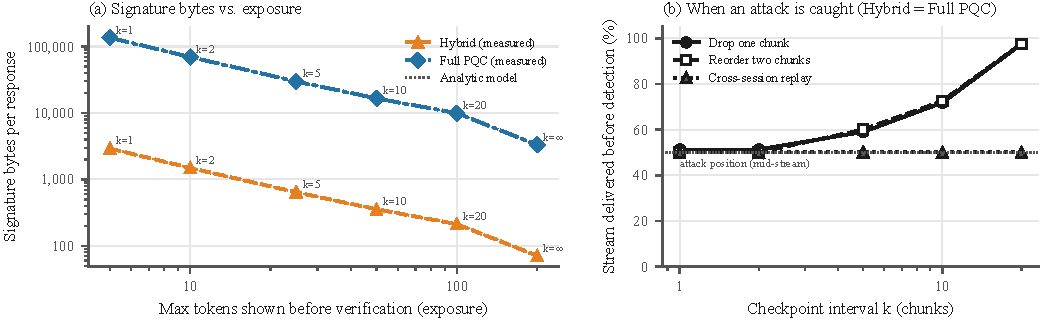
\includegraphics[width=\textwidth]{fig_checkpoint_frontier.pdf}
\caption{Checkpointed hash chains on Llama-3.2-3B (200-token responses, 5-token chunks). (a) Signature
bytes against exposure (most tokens displayed before verification); the measurements lie on the
analytic model. (b) Share of the stream delivered before a mid-stream drop, reorder, or cross-session
replay is detected; the dotted line marks the attack position.}
\label{fig:checkpoint}
\end{figure*}

\begin{table}[t]
\centering
\caption{Checkpointed hash-chain signing on Llama-3.2-3B (200-token responses, 5-token chunks): a signature every $k$ chunks plus the terminal one. Exposure = most tokens a client displays before a signature covers them (median over repetitions).}
\label{tab:checkpoint}
\setlength{\tabcolsep}{2.5pt}
\footnotesize
\begin{tabular}{@{}llrrrrr@{}}
\toprule
Config. & $k$ & Sigs & Bytes & Exp.\ (tok) & Lag (ms) & Sign+ver.\ (ms) \\
\midrule
Hybrid & 1 & 41 & 2,913 & 5 & 0 & 27.30 \\
 & 2 & 21 & 1,489 & 10 & 172 & 13.68 \\
 & 5 & 9 & 639 & 25 & 557 & 5.91 \\
 & 10 & 5 & 355 & 50 & 1,210 & 0.69 \\
 & 20 & 3 & 212 & 100 & 3,451 & 1.01 \\
 & $\infty$ & 1 & 71 & 200 & 5,298 & 0.65 \\
\addlinespace
Full PQC & 1 & 41 & 135,669 & 5 & 0 & 5.67 \\
 & 2 & 21 & 69,489 & 10 & 146 & 17.95 \\
 & 5 & 9 & 29,781 & 25 & 626 & 7.52 \\
 & 10 & 5 & 16,545 & 50 & 1,232 & 0.76 \\
 & 20 & 3 & 9,927 & 100 & 2,647 & 1.87 \\
 & $\infty$ & 1 & 3,309 & 200 & 5,570 & 0.57 \\
\bottomrule
\end{tabular}
\end{table}


\subsection{Harvest-Now-Decrypt-Later Exposure}\label{sec:res-hndl}
A passive adversary captures 209--433\,B per classical transaction and 1,265--4,503\,B per
post-quantum transaction (Fig.~\ref{fig:wirebytes}). Only the classical captures---RSA-OAEP and X25519
alike---become decryptable once a CRQC exists. Under streaming (Fig.~\ref{fig:streaminghndl}) the
decryptable volume $D$ grows linearly with response length for both classical key exchanges, at 11.4
bytes per generated token ($R^2{=}0.9997$, 50--585 tokens; the model ends longer requests early), of
which 5.8 bytes per token are recoverable plaintext and the rest is per-chunk AEAD framing. Under the
modeled attack, all three ML-KEM configurations have zero decryptable bytes at every length.

\begin{figure}[t]
\centering
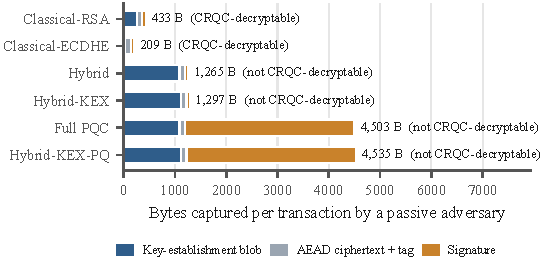
\includegraphics[width=\columnwidth]{fig_wire_bytes.pdf}
\caption{Bytes a passive adversary captures per transaction, by component. Larger post-quantum
captures are not decryptable by a future CRQC; the smaller classical ones are.}
\label{fig:wirebytes}
\end{figure}

\begin{figure}[t]
\centering
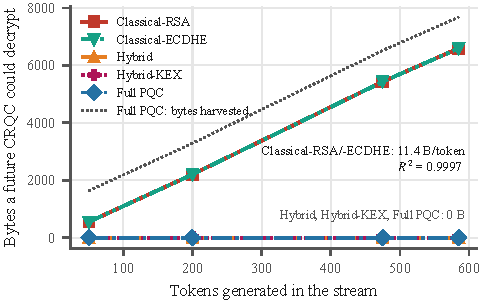
\includegraphics[width=\columnwidth]{fig_streaming_hndl.pdf}
\caption{Streaming HNDL exposure on Llama-3.2-3B. Under classical key exchange (RSA or X25519) the
bytes a future CRQC could decrypt grow by 11.4 per generated token; under every ML-KEM configuration
they stay at zero although more bytes are harvested.}
\label{fig:streaminghndl}
\end{figure}

\subsection{Active Tampering}\label{sec:res-mitm}
Every tampered response was rejected in every configuration (Table~\ref{tab:threats}). A flipped
ciphertext bit is caught by the AES-GCM tag in 0.007--0.008\,ms (median), before the signature is
examined; a flipped signature bit is caught by verification in 0.059\,ms (ML-DSA-65) to 0.083\,ms
(ECDSA P-256). All five sequence attacks were detected in every trial, in every configuration and
strategy. Per-chunk signing detects drop, reorder, duplicate, and cross-session replay at the affected
chunk (100\% mid-stream). Hash-chain detects replay immediately (the foreign chunk fails AEAD) and drop,
reorder, and duplicate at the end unless checkpoints are used (Section~\ref{sec:res-checkpoint}).
Truncation is detected by both strategies only at the end, through the missing signed terminal record;
without that record, as in a naive design, a truncated per-chunk stream would verify completely.

\begin{table}[t]
\centering
\caption{Tampering with single responses: one flipped bit per response, in the AEAD ciphertext or in the signature. Detection time is the rejecting check alone (median).}
\label{tab:threats}
\setlength{\tabcolsep}{4pt}
\footnotesize
\begin{tabular}{@{}llrrr@{}}
\toprule
Config. & Target & $n$ & Detected & Detection (ms) \\
\midrule
Classical-RSA & ciphertext & 100 & 100\% & 0.007 \\
Classical-RSA & signature & 100 & 100\% & 0.063 \\
Classical-ECDHE & ciphertext & 100 & 100\% & 0.008 \\
Classical-ECDHE & signature & 100 & 100\% & 0.083 \\
Hybrid & ciphertext & 100 & 100\% & 0.008 \\
Hybrid & signature & 100 & 100\% & 0.083 \\
Hybrid-KEX & ciphertext & 100 & 100\% & 0.008 \\
Hybrid-KEX & signature & 100 & 100\% & 0.082 \\
Full PQC & ciphertext & 100 & 100\% & 0.008 \\
Full PQC & signature & 100 & 100\% & 0.059 \\
Hybrid-KEX-PQ & ciphertext & 100 & 100\% & 0.009 \\
Hybrid-KEX-PQ & signature & 100 & 100\% & 0.058 \\
\bottomrule
\end{tabular}
\end{table}


% =============================================================================
\section{Ground-Truth Validation}\label{sec:validation}
All 75 tested NIST ACVP known-answer vectors pass (Table~\ref{tab:acvp_results}): our ML-KEM-768
key generation, encapsulation, and decapsulation reproduce the published outputs byte for byte, and
ML-DSA-65 verification returns the expected verdict on every tested vector. This checks the
correctness of our bindings on these vectors; it is not ACVP certification and does not cover ML-DSA
key generation or signing. Byte-exact ML-DSA-65 key and signature
reproduction is not possible through liboqs's public API, which exposes neither derandomized key
generation nor deterministic signing.

Signature-byte predictions of the analytic model matched the harness's measurements exactly for the
three strategies and, in the checkpoint sweep, for all twelve configuration--interval cells (for
example 41 ML-DSA-65 signatures, 135,669\,B, at $k{=}1$). Timing validation surfaced a genuine effect
rather than a confirmation: ECDSA P-256's first signing call in a fresh process took 7.7--9.3\,ms against
a 37.8--42.3\,\textmu s warm-loop mean, a 211--283$\times$ gap attributable to lazy OpenSSL backend
initialization, while ML-DSA-65 through our liboqs binding showed no such penalty. Correcting for this
cold-start effect reduced the two largest timing discrepancies from 281$\times$/297$\times$ to
1.33$\times$/1.41$\times$; a smaller residual (3--9$\times$) remains only partially explained.
Byte-overhead results are unaffected.

\begin{table}[t]
\caption{NIST ACVP known-answer-test results (75/75)}
\label{tab:acvp_results}
\centering
\footnotesize
\begin{tabular}{@{}L{4.2cm}cc@{}}
\toprule
Test & Result & Basis \\
\midrule
ML-KEM-768 keygen (derand., Alg.~16) & 25/25 & byte-exact \\
ML-KEM-768 encapsulation (Alg.~17) & 25/25 & byte-exact \\
ML-KEM-768 decapsulation (incl.\ 5 implicit-rej.) & 10/10 & byte-exact \\
ML-DSA-65 signature verification (Alg.~3) & 15/15 & correct verdict \\
\bottomrule
\end{tabular}
\end{table}

\begin{table}[t]
\centering
\caption{Primitive-level micro-benchmark (single process, warm loop). $n$ = timed iterations.}
\label{tab:primitives}
\setlength{\tabcolsep}{3pt}
\footnotesize
\begin{tabular}{@{}llrrrr@{}}
\toprule
Algorithm & Op. & $n$ & Median ($\mu$s) & p99 ($\mu$s) & ops/s \\
\midrule
ML-KEM-768 & KeyGen & 2000 & 10.2 & 12.5 & 98,357 \\
ML-KEM-768 & Encaps & 2000 & 11.5 & 14.7 & 86,640 \\
ML-KEM-768 & Decaps & 2000 & 13.1 & 15.0 & 76,190 \\
\addlinespace
X25519 & KeyGen & 2000 & 80.7 & 93.5 & 12,390 \\
X25519 & Exchange & 2000 & 137.2 & 150.1 & 7,288 \\
\addlinespace
RSA-2048 & KeyGen & 200 & 62,698.0 & 257,378.1 & 16 \\
RSA-2048 OAEP & Encrypt & 2000 & 24.3 & 27.3 & 41,237 \\
RSA-2048 OAEP & Decrypt & 2000 & 811.3 & 1,730.7 & 1,233 \\
\addlinespace
ML-DSA-65 & KeyGen & 2000 & 38.0 & 42.3 & 26,316 \\
ML-DSA-65 & Sign & 2000 & 67.9 & 246.1 & 14,733 \\
ML-DSA-65 & Verify & 2000 & 35.5 & 40.8 & 28,202 \\
\addlinespace
ECDSA P-256 & KeyGen & 2000 & 15.5 & 18.5 & 64,687 \\
ECDSA P-256 & Sign & 2000 & 21.0 & 23.7 & 47,619 \\
ECDSA P-256 & Verify & 2000 & 46.3 & 54.2 & 21,602 \\
\bottomrule
\end{tabular}
\end{table}


\begin{table}[t]
\centering
\caption{Software and hardware environment, captured automatically at run time.}
\label{tab:environment}
\footnotesize
\setlength{\tabcolsep}{3pt}
\begin{tabular}{@{}ll@{}}
\toprule
Component & Version \\
\midrule
Host & Apple M3, 8 cores, 16\,GB \\
OS & macOS 26.6.2 \\
Python & 3.13.5 \\
FastAPI / Uvicorn / httpx & 0.141.1 / 0.52.4 / 0.28.1 \\
cryptography / OpenSSL & 50.0.0 / 4.0.1 \\
liboqs (commit) & 8979276ad1eb \\
NumPy / SciPy / pandas & 2.5.2 / 1.18.1 / 3.0.5 \\
scikit-learn & 1.9.0 \\
llama-cpp-python (Metal) & 0.3.35 \\
LLM file & Llama-3.2-3B-Instruct-Q4\_K\_M.gguf \\
LLM SHA-256 (prefix) & 6c1a2b4116103267 \\
Classifier SHA-256 (prefix) & 68b46ef7e1efce32 \\
\bottomrule
\end{tabular}
\end{table}


\begin{figure*}[t]
\centering
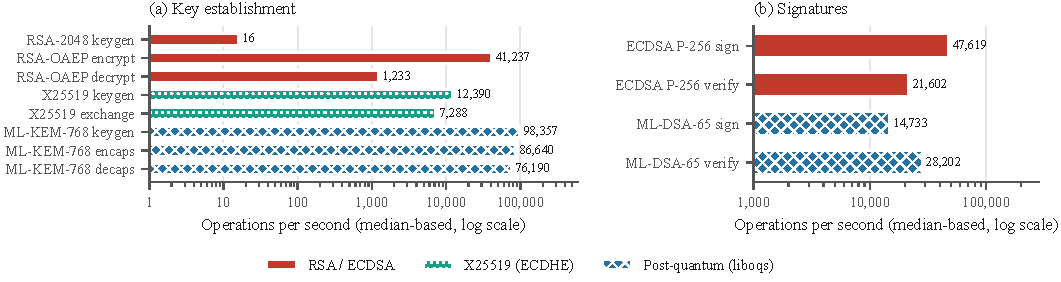
\includegraphics[width=\textwidth]{fig_primitive_throughput.pdf}
\caption{Primitive throughput (single process, warm loop, median-based). (a) Key establishment, log
scale: RSA-2048 key generation is 6,167$\times$ slower than ML-KEM-768 key generation, and ML-KEM-768 is
also cheaper than X25519. (b) Signatures: ML-DSA-65 verification is 1.31$\times$ faster than ECDSA
P-256 despite a $\approx$47$\times$ larger signature.}
\label{fig:primitives}
\end{figure*}

% =============================================================================
\section{Discussion and Decision Framework}
We construct a weighted composite score,
\begin{equation}
\text{composite} = w_{\text{sec}}\cdot S - w_{\text{perf}}\cdot O,
\end{equation}
where $O$ is the end-to-end latency overhead versus the control and $S$ an explicit ordinal security
score: 0.0 for Classical-RSA and Classical-ECDHE (no quantum resistance on either axis), 0.8 for Hybrid
and Hybrid-KEX (post-quantum key exchange prevents the modeled HNDL key recovery; the ECDSA signature remains classically
vulnerable, a materially smaller risk because signatures protect real-time integrity rather than the
confidentiality of harvested traffic), and 1.0 for Full PQC. Rather than collapse this judgment into
one number, Table~\ref{tab:tradeoff} reports the matrix at three weightings. Full PQC scores highest in
most cells because its overhead matches Hybrid's while its security score is higher; the cells at 100
connections inherit the queueing bimodality of Section~\ref{sec:res-concurrency} and should not be
used to rank configurations.

\begin{table*}[t]
\centering
\caption{Weighted composite score $w_{sec}\cdot S - w_{perf}\cdot O$ (higher is better), where $S$ is the security score (Classical 0, Hybrid 0.8, Full PQC 1.0) and $O$ the end-to-end latency overhead versus Control. Bold: best at that weighting and concurrency; fail: every request failed; n/a: not measured.}
\label{tab:tradeoff}
\setlength{\tabcolsep}{4pt}
\begin{tabular}{@{}lrrrrrrrrr@{}}
\toprule
 & \multicolumn{3}{c}{Security ($w_{sec}{=}0.8$)} & \multicolumn{3}{c}{Balanced ($w_{sec}{=}0.5$)} & \multicolumn{3}{c}{Performance ($w_{sec}{=}0.2$)} \\
\cmidrule(lr){2-4}\cmidrule(lr){5-7}\cmidrule(lr){8-10}
Config. & 10 & 100 & 1,000 & 10 & 100 & 1,000 & 10 & 100 & 1,000 \\
\midrule
Classical-RSA & $-0.17$ & $-0.31$ & $-0.45$ & $-0.43$ & $-0.76$ & $-1.13$ & $-0.69$ & $-1.22$ & $-1.81$ \\
Classical-ECDHE & $-0.01$ & $-0.10$ & $-0.22$ & $-0.02$ & $-0.24$ & $-0.56$ & $-0.04$ & $-0.38$ & $-0.90$ \\
Hybrid & $+0.63$ & $+0.62$ & $+0.42$ & $+0.38$ & $\mathbf{+0.35}$ & $-0.14$ & $+0.12$ & $\mathbf{+0.07}$ & $-0.71$ \\
Hybrid-KEX & $+0.62$ & $+0.55$ & $+0.40$ & $+0.36$ & $+0.18$ & $-0.19$ & $+0.10$ & $-0.20$ & $-0.78$ \\
Full PQC & $\mathbf{+0.79}$ & $\mathbf{+0.72}$ & $\mathbf{+0.58}$ & $\mathbf{+0.48}$ & $+0.29$ & $\mathbf{-0.06}$ & $\mathbf{+0.17}$ & $-0.13$ & $\mathbf{-0.69}$ \\
\bottomrule
\end{tabular}
\end{table*}


\paragraph*{Hypotheses} \textbf{H1} (bounded post-quantum overhead) is supported: Hybrid and Full PQC
are equivalent to Classical-ECDHE within $\pm5\%$ at 10 and 1,000 connections, their cryptographic
overhead over the matched protocol is 1.3--2.3\,ms at 10 connections, and in the byte-level emulation
they add at most 5.7\,ms of handshake time; at 100 connections queueing bimodality prevents a
conclusion. \textbf{H2} (Hybrid captures Full PQC's HNDL benefit at lower cost) is supported on HNDL,
where both have zero decryptable bytes under the modeled attack, but not on cost: Full PQC is no slower
than Hybrid in any non-streaming experiment and costs more only in signature bytes when many signatures
are sent. \textbf{H3} (categorically different decryptability) is demonstrated: classical exposure
grows linearly with streamed tokens, ML-KEM-based exposure stays at zero. \textbf{H4} (ML-DSA-65
verification not slower than ECDSA P-256) is confirmed: 28,202 versus 21,602 verifications/s
(1.31$\times$).

% =============================================================================
\section{Recommendations}

\paragraph*{Key establishment} Within the evaluated threat model, migrating from X25519 to ML-KEM-768
removes the modeled HNDL exposure at no practically significant latency cost in our workload (equivalent
within $\pm5\%$ at 10 and 1,000 connections), about 5\,ms of handshake time on a slow emulated link, and
0--2\% once sessions are reused. Where hedging against an ML-KEM weakness matters, the
X25519MLKEM768 hybrid cost about 3\,ms more than ML-KEM alone at 10 connections in our implementation.
Per-handshake RSA key generation should be avoided: it occupied 4--5 CPU cores at modest load and fails
when cores run out.

\paragraph*{Signatures} ML-DSA-65 verification is faster than ECDSA P-256, so Full PQC added no
practically significant latency for single-shot responses. Its 3,309\,B signature matters only where
many signatures are sent, which in practice means streaming.

\paragraph*{Streaming} Use hash-chained signing with checkpoints, bind session context and a signed
end-of-stream record (Section~\ref{sec:binding}), and choose $k$ from the exposure the application can
tolerate: $k{=}\infty$ (one signature; the response is unverified until it ends) for low-risk display,
small $k$ where a user must not act on unverified text. With ML-DSA-65, $k{=}5$ bounds exposure to 25
tokens for 29,781\,B per 200-token response, against 135,669\,B for per-chunk signing. Buffer-and-sign is
justified only when chunk-count and timing metadata must be hidden~\cite{weiss2024keylogging}, at a
38--41$\times$ time-to-first-token penalty.

\begin{table}[t]
\centering
\caption{Recommendation summary}
\label{tab:recommendations}
\setlength{\tabcolsep}{3pt}
\footnotesize
\begin{tabular}{@{}L{2.9cm}L{4.9cm}@{}}
\toprule
Scenario & Recommendation \\
\midrule
Any inference API & Key exchange: ML-KEM-768, or X25519MLKEM768 to hedge against an ML-KEM break \\
Non-streaming responses & ECDSA P-256 or ML-DSA-65 (no latency difference) \\
Streaming, display-only & Hash-chain, $k=\infty$ \\
Streaming, actionable output & Hash-chain with small $k$ (e.g.\ $k=5$: 25-token exposure) \\
Any streaming & Bind session context; sign an end-of-stream record \\
Long-term non-repudiation & ML-DSA-65 signatures (Full PQC) \\
Metadata-sensitive streaming & Buffer-and-sign \\
Legacy RSA key transport & Migrate away \\
\bottomrule
\end{tabular}
\end{table}

% =============================================================================
\section{Limitations}
\begin{itemize}
  \item \textbf{Single host.} All measurements come from one machine (Apple M3, 8 cores, 16\,GB). The
  load generator and server share its CPU, which matters most at 1,000 connections. Relative
  comparisons between configurations are the intended result; absolute latencies are host-specific.
  \item \textbf{Application-layer protocol, not TLS.} PQ-Shield's handshake is a purpose-built
  protocol. Its default fresh key exchange per transaction isolates the asymmetric primitive and is a
  worst case; Section~\ref{sec:sessions} measures the amortized case, but not TLS's own resumption
  mechanisms (PSK, 0-RTT). Server keys are not certificate-authenticated, so it is not a substitute for
  authenticated TLS.
  \item \textbf{Network emulation is byte-level.} The proxy models propagation delay and bandwidth but
  not TCP congestion control, loss, or MTU fragmentation. Results are a lower bound on post-quantum
  network cost; packet-level studies~\cite{paquin2020benchmarking,sikeridis2020authentication} remain
  the reference for lossy links.
  \item \textbf{Classical-RSA is a worst case.} Its per-handshake RSA-2048 key generation does not
  reflect production practice; its failure under load is a property of that design, contrasted with
  the realistic Classical-ECDHE baseline.
  \item \textbf{Hybrid-KEX measured separately.} Configuration B$'$ was added after the main concurrency
  sweep; its concurrency results come from a supplementary run on the same host and day. Its streaming
  behaviour was measured with the others; its signature path is identical to Hybrid's.
  \item \textbf{Workloads.} The \texttt{image\_cnn} profile uses an untrained fixed-weight network and
  the \texttt{embedding}/\texttt{llm\_completion} profiles are synthetic; they probe payload shape and
  size, not model behaviour. Streaming uses one quantized 3B-parameter model, which may end a stream
  before the requested length, so streaming HNDL is reported against tokens actually generated.
  \item \textbf{Queueing at 100 connections.} At 100 connections the protected configurations switch
  between two latency regimes across repetitions while both controls do not; with client and server on
  one host we cannot fully explain this, and we do not rank the non-RSA configurations at that level. A
  separate load-generator host would resolve it.
  \item \textbf{Thermal drift in streaming.} Over the 18-minute streaming sweep, generation slowed from
  $\approx$40 to $\approx$33 tokens/s on the fanless host. Strategy order was shuffled within each
  configuration, so strategy comparisons are unbiased, but streaming times are not compared across
  configurations; signature bytes are unaffected.
  \item \textbf{Repetitions.} Five repetitions per cell bound the precision of between-run
  comparisons; with repetition medians as the unit, the smallest attainable $p$ is 0.008, and
  confidence intervals at 100 connections are wide because of queueing bimodality.
  \item \textbf{Timing-validation residual.} A 3--9$\times$ gap between predicted and measured streaming
  \emph{signing time} for some strategy--configuration pairs remains only partially explained;
  signature-\emph{byte} predictions match exactly.
\end{itemize}

% =============================================================================
\section{Conclusion and Future Work}
Measured on a real inference service through an application-layer emulation, the answers to the
practical questions are as follows; each holds under our threat model and on our single host.

\paragraph*{Strongest security} Full PQC (ML-KEM-768 with ML-DSA-65) is the only evaluated
configuration whose key establishment and signatures both resist known quantum attacks. Hybrid-KEX
offers the most conservative key establishment, since X25519MLKEM768 stays secure unless both of its
components are broken, but its ECDSA signatures remain classically vulnerable. Combining
X25519MLKEM768 with ML-DSA-65 would dominate both; we did not measure it.

\paragraph*{Best performance} Among realistic configurations there is no single fastest one: Full PQC,
Hybrid, and Classical-ECDHE are statistically equivalent within $\pm5\%$ at 10 and 1,000 connections,
with cryptographic overheads of 1.3--2.7\,ms per 92\,ms transaction; Hybrid-KEX adds about 5\,ms.
Classical-RSA with per-transaction key generation is clearly the slowest. When many signatures are
sent---per-chunk streaming or frequent checkpoints---the ECDSA-signed configurations are cheapest in
bytes, by a factor of about 47 per signature.

\paragraph*{Best balance} For non-streaming inference APIs, and for streaming with hash-chained signing
and few checkpoints, Full PQC offers the best balance: the strongest security at no practically
significant latency cost, and it scores highest in the weighted decision matrix in 7 of 9 cells. When
every chunk must be signed or checkpoints are frequent, Hybrid (or Hybrid-KEX) is the better balance:
at $k{=}1$ a 200-token response carries 2,913\,B of ECDSA signatures instead of 135,669\,B of ML-DSA-65.

\paragraph*{What the answer depends on} \emph{Streaming:} the signing schedule, not the key exchange,
determines the post-quantum cost, through the number of signatures sent. \emph{Session reuse:} reusing
one key exchange for 100 requests reduced every non-RSA configuration's overhead to 0--2\%, making the
key-exchange choice nearly free. \emph{Threat model:} if only HNDL confidentiality matters, Hybrid
suffices; quantum-resistant signatures or long-term non-repudiation require Full PQC; hedging against a
break of ML-KEM itself favours Hybrid-KEX. \emph{Network:} slow links add a few milliseconds of handshake
time for ML-KEM, more under real packet loss than our byte-level emulation shows.

Future work includes a separate load-generator host and packet-level network measurements, a
TLS-native implementation with certificate authentication and resumption, mid-stream rekeying to bound
HNDL exposure per session, the X25519MLKEM768 with ML-DSA-65 combination, and a trained, larger-scale
vision workload.

% TODO(authors): Dr. Nivitha K is a co-author, so she is not thanked here; add funding or other
% acknowledgments if any.
\section*{Acknowledgment}
The authors thank the faculty and technical staff of the School of Computer Science and Engineering
(SCOPE), Vellore Institute of Technology, Vellore, for the resources and infrastructure used in this
study, and the open-source cryptographic and machine-learning communities, whose tools and standards
supported its implementation, validation, and evaluation.

% =============================================================================
\begin{thebibliography}{99}

\bibitem{abbasi2025benchmark} M. Abbasi, F. Cardoso, P. V\'az, J. Silva, and P. Martins, ``A practical
performance benchmark of post-quantum cryptography across heterogeneous computing environments,''
\textit{Cryptography}, vol.~9, no.~2, art.~32, 2025, doi: 10.3390/cryptography9020032.

\bibitem{demir2025industry} E. D. Demir, B. Bilgin, and M. C. Onbasli, ``Performance analysis and
industry deployment of post-quantum cryptography algorithms,'' arXiv:2503.12952, 2025.

\bibitem{egbuagha2025practice} O. Egbuagha and E. Ikwunna, ``Post-quantum cryptography in practice: A
literature review of protocol-level transitions and readiness,'' IACR Cryptology ePrint Archive, Paper
2025/1668, 2025.

\bibitem{pote2025evaluation} P. Pote and R. Bansode, ``Performance evaluation of post-quantum
cryptography: A comprehensive framework for experimental analysis,'' \textit{J. Inf. Syst. Eng.
Manage.}, vol.~10, no.~9s, pp.~548--556, 2025, doi: 10.52783/jisem.v10i9s.1253.

\bibitem{shaw2026quantumsafe} A. Shaw, ``quantum-safe: Bridging the post-quantum production gap with a
hybrid-by-default Python cryptography library,'' arXiv:2605.17061, 2026.

\bibitem{montenegro2026framework} J. A. Montenegro, R. Rios, and J. Lopez-Cerezo, ``A performance
evaluation framework for post-quantum TLS,'' \textit{Future Gener. Comput. Syst.}, vol.~175,
art.~108062, 2026, doi: 10.1016/j.future.2025.108062.

\bibitem{chhetri2025survey} G. Chhetri, S. Somvanshi, P. Hebli, S. Brotee, and S. Das, ``Post-quantum
cryptography and quantum-safe security: A comprehensive survey,'' arXiv:2510.10436, 2025.

\bibitem{faval2026mobile} R. A. Faval, R. Moreira, and F. de Oliveira Silva, ``Empowering mobile
networks security resilience by using post-quantum cryptography,'' arXiv:2603.28626, 2026.

\bibitem{kudaloor2026sixg} A. Kudaloor and A. Aijaz, ``Toward quantum-safe 6G: Experimental evaluation
of post-quantum cryptography techniques,'' \textit{IEEE Commun. Standards Mag.}, accepted, 2026,
arXiv:2605.06881.

\bibitem{song2019privacy} L. Song, R. Shokri, and P. Mittal, ``Privacy risks of securing machine
learning models against adversarial examples,'' in \textit{Proc. ACM SIGSAC Conf. Comput. Commun.
Secur. (CCS)}, 2019, pp.~241--257.

\bibitem{tidjon2022threat} L. N. Tidjon and F. Khomh, ``Threat assessment in machine learning based
systems,'' arXiv:2207.00091, 2022.

\bibitem{ahmed2025libraries} N. Ahmed, L. Zhang, and A. Gangopadhyay, ``A survey of post-quantum
cryptography support in cryptographic libraries,'' in \textit{Proc. IEEE Int. Conf. Quantum Comput.
Eng. (QCE)}, 2025, arXiv:2508.16078.

\bibitem{blancoromero2026hndl} J. Blanco-Romero, F. Almenares Mendoza, C. Garc\'ia Rubio, C. Campo,
and D. D\'iaz S\'anchez, ``On the practical feasibility of harvest-now, decrypt-later attacks,''
arXiv:2603.01091, 2026.

\bibitem{gomezcambronero2026layered} D. G\'omez-Cambronero, D. Munteanu, and A. I.
Gonz\'alez-Tablas, ``Layered performance analysis of TLS 1.3 handshakes: Classical, hybrid, and pure
post-quantum key exchange,'' arXiv:2603.11006, 2026.

\bibitem{schemitt2025blockchain} A. G. Schemitt, H. F. da Silva, R. C. Lunardi, D. Kreutz, R. B.
Mansilha, and A. F. Zorzo, ``Assessing the impact of post-quantum digital signature algorithms on
blockchains,'' in \textit{Proc. IEEE Int. Conf. Trust, Secur. Privacy Comput. Commun. (TrustCom)},
2025, arXiv:2510.09271.

\bibitem{fips203} National Institute of Standards and Technology, ``Module-lattice-based
key-encapsulation mechanism standard,'' FIPS PUB 203, Aug. 2024, doi: 10.6028/NIST.FIPS.203.

\bibitem{fips204} National Institute of Standards and Technology, ``Module-lattice-based digital
signature standard,'' FIPS PUB 204, Aug. 2024, doi: 10.6028/NIST.FIPS.204.

\bibitem{acvp} National Institute of Standards and Technology, ``Automated Cryptographic Validation
Protocol (ACVP) server and test vectors,'' 2024. [Online]. Available:
\url{https://github.com/usnistgov/ACVP-Server}

\bibitem{rfc8446} E. Rescorla, ``The Transport Layer Security (TLS) protocol version 1.3,'' IETF RFC
8446, Aug. 2018.

\bibitem{ietf-ecdhe-mlkem} K. Kwiatkowski, P. Kampanakis, B. Westerbaan, and D. Stebila,
``Post-quantum hybrid ECDHE-MLKEM key agreement for TLSv1.3,'' IETF Internet-Draft
draft-ietf-tls-ecdhe-mlkem-05, May 2026.

\bibitem{shor1997} P. W. Shor, ``Polynomial-time algorithms for prime factorization and discrete
logarithms on a quantum computer,'' \textit{SIAM J. Comput.}, vol.~26, no.~5, pp.~1484--1509, 1997.

\bibitem{mosca2018ready} M. Mosca, ``Cybersecurity in an era with quantum computers: Will we be
ready?'' \textit{IEEE Secur. Privacy}, vol.~16, no.~5, pp.~38--41, 2018.

\bibitem{stebila2016oqs} D. Stebila and M. Mosca, ``Post-quantum key exchange for the Internet and the
Open Quantum Safe project,'' in \textit{Selected Areas in Cryptography -- SAC 2016}, ser. LNCS,
vol.~10532. Springer, 2017, pp.~14--37.

\bibitem{paquin2020benchmarking} C. Paquin, D. Stebila, and G. Tamvada, ``Benchmarking post-quantum
cryptography in TLS,'' in \textit{Post-Quantum Cryptography -- PQCrypto 2020}, ser. LNCS, vol.~12100.
Springer, 2020, pp.~72--91.

\bibitem{sikeridis2020authentication} D. Sikeridis, P. Kampanakis, and M. Devetsikiotis,
``Post-quantum authentication in TLS 1.3: A performance study,'' in \textit{Proc. Netw. Distrib. Syst.
Secur. Symp. (NDSS)}, 2020.

\bibitem{gennaro1997streams} R. Gennaro and P. Rohatgi, ``How to sign digital streams,'' in
\textit{Advances in Cryptology -- CRYPTO '97}, ser. LNCS, vol.~1294. Springer, 1997, pp.~180--197.

\bibitem{wong1999flows} C. K. Wong and S. S. Lam, ``Digital signatures for flows and multicasts,''
\textit{IEEE/ACM Trans. Netw.}, vol.~7, no.~4, pp.~502--513, 1999.

\bibitem{perrig2000tesla} A. Perrig, R. Canetti, J. D. Tygar, and D. Song, ``Efficient authentication
and signing of multicast streams over lossy channels,'' in \textit{Proc. IEEE Symp. Secur. Privacy},
2000, pp.~56--73.

\bibitem{weiss2024keylogging} R. Weiss, D. Ayzenshteyn, G. Amit, and Y. Mirsky, ``What was your prompt?
A remote keylogging attack on AI assistants,'' in \textit{Proc. 33rd USENIX Secur. Symp.}, 2024,
pp.~3367--3384.

\end{thebibliography}

\end{document}
